% Created 2026-09-20 Sun 13:15
% Intended LaTeX compiler: xelatex
\documentclass[14pt]{extarticle}

\usepackage{amsmath}
\usepackage{fontspec}
\usepackage{graphicx}
\usepackage{longtable}
\usepackage{wrapfig}
\usepackage{rotating}
\usepackage[normalem]{ulem}
\usepackage{capt-of}
\usepackage{hyperref}
\usepackage{fontspec}
\usepackage{amsmath}
\usepackage{amssymb}
\usepackage{amsfonts}
\usepackage{geometry}
\geometry{left=20mm, right=15mm, top=15mm, bottom=15mm}
\setmainfont{Times New Roman}
\setsansfont{Times New Roman}
\setmonofont{"Consolas-with-Yahei"}
\newfontfamily\codefont{"Consolas-with-Yahei"}[Scale=0.88]
\usepackage{seqsplit}
\renewcommand{\texttt}[1]{{\codefont \seqsplit{#1}}}
\newfontfamily\cyrillicfont{Times New Roman}[Script=Cyrillic]
\newfontfamily\cyrillicfontsf{Times New Roman}[Script=Cyrillic]
\newfontfamily\cyrillicfonttt{"Consolas-with-Yahei"}[Script=Cyrillic]
\usepackage{setspace}
\setstretch{1.15}
\usepackage{titlesec}
\titleformat{\section}{\fontsize{16}{24}\selectfont\bfseries\raggedright}{}{0em}{}
\titleformat{\subsection}{\fontsize{16}{24}\selectfont\bfseries\raggedright}{}{0em}{}
\titleformat{\subsubsection}{\fontsize{16}{24}\selectfont\bfseries\raggedright}{}{0em}{}
\titlespacing*{\section}{0pt}{24pt}{12pt}
\titlespacing*{\subsection}{0pt}{18pt}{6pt}
\titlespacing*{\subsubsection}{0pt}{12pt}{6pt}
\usepackage[labelsep=period]{caption}
\DeclareCaptionFont{captionfont}{\fontsize{12}{12}\selectfont}
\captionsetup{font=captionfont}
\captionsetup[figure]{name={Рисунок}, labelsep=period, font={captionfont,it}, justification=centering, singlelinecheck=false, skip=6pt}
\captionsetup[table]{name={Таблица}, labelsep=period, font={captionfont,it}, justification=raggedright, singlelinecheck=false, skip=6pt}
\renewcommand{\contentsname}{Содержание}
\renewcommand{\figurename}{Рисунок}
\renewcommand{\tablename}{Таблица}
\usepackage{float}
\usepackage{xcolor}
\usepackage{booktabs}
\usepackage{microtype}
\setlength{\emergencystretch}{3em}
\tolerance=2000
\usepackage{indentfirst}
\setlength{\parindent}{1.25cm}
\setlength{\parskip}{0pt}
\usepackage[newfloat]{minted}
\setminted{fontsize=\fontsize{12}{12}\selectfont, frame=single, tabsize=2, breaklines}
\SetupFloatingEnvironment{listing}{name={Листинг}}
\captionsetup[listing]{name={Листинг}, labelsep=period, font={captionfont,it}, justification=raggedright, singlelinecheck=false}
\date{}
\usepackage{fancyhdr}
\pagestyle{fancy}
\fancyhf{}
\fancyfoot[C]{\thepage}
\renewcommand{\headrulewidth}{0pt}
\hypersetup{colorlinks=true, linkcolor=black, urlcolor=blue, citecolor=black}
\author{Фриев Д.С.}
\date{2026}
\title{Создание приложений вероятностного моделирования}
\hypersetup{
 pdfauthor={Фриев Д.С.},
 pdftitle={},
 pdfkeywords={},
 pdfsubject={},
 pdfcreator={},
 pdflang={English}}
\usepackage{biblatex}

\begin{document}

\begin{titlepage}
\thispagestyle{empty}
\begin{center}
{\fontsize{14}{18}\selectfont
МИНИСТЕРСТВО НАУКИ И ВЫСШЕГО ОБРАЗОВАНИЯ РФ\par
\vspace{4mm}
РГУ им.\ А.Н.~Косыгина (Технологии. Дизайн. Искусство)\par
\vspace{4mm}
Институт Информационных технологий и цифровой трансформации\par
\vspace{4mm}
Кафедра <<Искусственного интеллекта, прикладной математики и программирования>>\par
}
\vspace{20mm}
{\fontsize{16}{24}\selectfont\bfseries Курсовая работа\par}
\vspace{6mm}
{\fontsize{16}{24}\selectfont\bfseries по предмету <<Вероятностное моделирование процессов и систем>>\par}
\vspace{6mm}
{\fontsize{16}{24}\selectfont\bfseries на тему\par}
\vspace{4mm}
{\fontsize{16}{24}\selectfont\bfseries <<Создание приложений вероятностного моделирования>>\par}
\vspace{30mm}
\begin{flushleft}
{\fontsize{14}{18}\selectfont
\hspace{60mm}Выполнил: студент группы ИТПМ-124\par
\hspace{60mm}Фриев Д.С.\par
\vspace{6mm}
\hspace{60mm}Научный руководитель:\par
\hspace{60mm}доцент кафедры ИИПМиП\par
\hspace{60mm}Романенков А.М.\par
}
\end{flushleft}
\vfill
{\fontsize{14}{18}\selectfont Москва --- 2026\par}
\end{center}
\end{titlepage}

\tableofcontents
\clearpage
\section{Введение}
\label{sec:org1c7cd5a}

\subsection{Цель и задачи}
\label{sec:orgd474bf5}

Цель работы --- программная реализация комплекса задач вероятностного моделирования. Для достижения цели необходимо решить следующие задачи:

\begin{itemize}
\item разработать математические модели для каждого задания;
\item продумать и создать архитектуру приложений;
\item реализовать пользовательский интерфейс для управления параметрами моделирования;
\item провести численные эксперименты и сравнить эмпирические результаты с теоретическими.
\end{itemize}
\subsection{Структура пояснительной записки}
\label{sec:org0f3a2c7}

Документ имеет следующую структуру:

\begin{itemize}
\item введение;
\item теоретические основы вероятностного моделирования;
\item описание задач с подробностями их реализации;
\item список использованных источников;
\item приложение со ссылкой на репозиторий исходного кода.
\end{itemize}

\clearpage
\section{Теоретическая часть}
\label{sec:org2ff3332}

\subsection{Законы распределения случайных величин}
\label{sec:org6b63750}

Во всех задачах работы моделирование основано на генерации значений случайных величин с заданными законами распределения. Ниже приведены распределения, используемые в программной реализации.

\textbf{Дискретное равномерное распределение.}

$$P(X = x_i) = \frac{1}{n}, \quad i = 1, \ldots, n$$

Случайная величина принимает \(n\) значений с равными вероятностями. Применяется для равновероятного выбора элементов из конечного множества: выбор символа из алфавита (задача~1), выбор направления блуждания (задачи~4,~6,~7), выбор монеты (задача~10), равномерное распределение положения и угла иглы (задача~12).

\textbf{Схема Бернулли и биномиальное распределение.}

$$P(X = k) = \binom{n}{k} p^{k} (1-p)^{n-k}, \quad k = 0, \ldots, n$$

Биномиальное распределение моделирует число успехов в \(n\) независимых испытаниях Бернулли с вероятностью успеха \(p\). Используется в задаче~8 (число попаданий при обстреле бочки) и как один из законов распределения шага блуждания в задачах~4,~6,~7. Частный случай \(n = 1\) --- распределение Бернулли --- применяется в задачах~2,~8,~10 для моделирования бинарных случайных событий (заражение, попадание, орёл).

\textbf{Усечённое геометрическое распределение.}

$$P(X = k) = \frac{p(1-p)^k}{\sum_{i=0}^{n-1} p(1-p)^i}, \quad k = 0, \ldots, n-1$$

Геометрическое распределение описывает число неудач до первого успеха. В работе используется его усечённая версия для генерации значений шага блуждания с убывающей вероятностью в задачах~4,~6,~7.

\clearpage

\textbf{Дискретное треугольное распределение.}

$$P(X = x_k) \propto \begin{cases} \dfrac{2(x_k - a)}{(c-a)(b-a)}, & a \le x_k \le b, \\[6pt] \dfrac{2(c - x_k)}{(c-a)(c-b)}, & b \le x_k \le c \end{cases}$$

Треугольное распределение применяется в задачах~4,~6,~7 как один из законов для генерации шага или направления. Непрерывное треугольное распределение \(\operatorname{Tri}(a,b,c)\) дискретизируется округлением до ближайшего допустимого значения.

\textbf{Непрерывное равномерное распределение.}

$$f(x) = \begin{cases} \dfrac{1}{b-a}, & x \in [a, b], \\[6pt] 0, & x \notin [a, b] \end{cases}$$

Непрерывное равномерное распределение задаётся плотностью вероятности, постоянной на отрезке \([a, b]\). Величина \(U \sim U(0,1)\) является базовой для генерации всех остальных распределений, поскольку любое преобразование случайной величины \(U\) даёт новую случайную величину с заданным законом. В работе \(U(0,1)\) используется в задаче~5 для генерации символов кластера по заданному распределению на алфавите.
\subsection{Метод Монте-Карло}
\label{sec:orgfe34f4f}

Метод Монте-Карло --- численный метод, основанный на многократной реализации случайного процесса с последующим усреднением.
Пусть \(\nu_n\) --- число появлений события \(A\) в \(n\) независимых испытаниях, и \(p = P(A)\) --- теоретическая вероятность. Согласно \textbf{теореме Бернулли}, для любого \(\varepsilon > 0\):

$$\lim_{n \to \infty} P\!\left( \left| \frac{\nu_n}{n} - p \right| < \varepsilon \right) = 1$$

Относительная частота \(\hat{p}_n = \nu_n / n\) сходится по вероятности к \(p\) при росте числа испытаний. Это фундаментальное утверждение оправдывает применение метода Монте-Карло: чем больше экспериментов проведено, тем точнее эмпирическая оценка.

\clearpage
\section{Практическая часть}
\label{sec:org0cd9751}

\subsection{Задача 1. Выбор символа из алфавита}
\label{sec:org750d5d2}

Из упорядоченного алфавита, содержащего \(N\) различных символов, последовательно выбирают два символа: сначала один, затем --- один из оставшихся. Все исходы считаются равновероятными. Требуется определить вероятность того, что в первый раз, во второй раз и оба раза будет выбран символ с чётным номером. Индексация элементов алфавита начинается с \(1\). Рассматриваются два варианта нумерации после первой выборки: а) индексы оставшихся элементов не изменяются; б) индексы изменяются (переиндексируются начиная с \(1\)).
\subsubsection{Аналитическое решение}
\label{sec:org08864cf}

Пусть алфавит содержит \(N\) символов с номерами от \(1\) до \(N\). Число чётных номеров равно \(\lfloor N/2 \rfloor\). Первый символ выбирается равновероятно из всех \(N\) элементов.

\textbf{Случай а) --- фиксированные индексы.}

$$P(\text{первый чётный}) = \frac{\lfloor N/2 \rfloor}{N}$$

При фиксированных индексах после удаления первого элемента оставшиеся \(N-1\) символов сохраняют свои номера. Вероятность того, что второй выбранный символ имеет чётный номер, зависит от чётности первого:

$$P(\text{второй чётный}) = \frac{\lfloor N/2 \rfloor}{N} \cdot \frac{\lfloor N/2 \rfloor - 1}{N-1} + \frac{\lceil N/2 \rceil}{N} \cdot \frac{\lfloor N/2 \rfloor}{N-1}$$

$$P(\text{оба чётных}) = \frac{\lfloor N/2 \rfloor}{N} \cdot \frac{\lfloor N/2 \rfloor - 1}{N - 1}$$

\textbf{Случай б) --- переиндексация после первой выборки.}

После удаления первого элемента оставшиеся \(N-1\) символов получают новые порядковые номера от \(1\) до \(N-1\). Число чётных позиций среди \(N-1\) элементов равно \(\lfloor (N-1)/2 \rfloor\).

$$P(\text{первый чётный}) = \frac{\lfloor N/2 \rfloor}{N}$$

$$P(\text{второй чётный}) = \frac{\lfloor (N-1)/2 \rfloor}{N-1}$$

$$P(\text{оба чётных}) = \frac{\lfloor N/2 \rfloor}{N} \cdot \frac{\lfloor (N-1)/2 \rfloor}{N-1}$$
\subsubsection{Эмпирическая проверка}
\label{sec:orgca83fdb}

Программа принимает два параметра командной строки: мощность алфавита \(N\) и количество экспериментов \(C\). Для генерации псевдослучайных чисел используется Вихрь Мерсенна (\texttt{std::mt19937}). Запуск серии экспериментов выполняется через вспомогательный класс \texttt{TaskRunner}.

\begin{listing}[htbp]
\caption{Эксперимент с фиксированными индексами}
\begin{minted}[]{cpp}
auto experiment_fixed_indices = [alphabet_size](auto& rng) {
    std::uniform_int_distribution<size_t> dist1(1, alphabet_size);
    size_t first = dist1(rng);

    std::vector<size_t> remaining;
    remaining.reserve(alphabet_size - 1);
    for (size_t i = 1; i <= alphabet_size; i++) {
        if (i != first) remaining.push_back(i);
    }

    std::uniform_int_distribution<size_t> dist2(0, remaining.size() - 1);
    size_t second = remaining[dist2(rng)];

    return Outcome{first % 2 == 0, second % 2 == 0};
};
\end{minted}
\end{listing}

\begin{listing}[htbp]
\caption{Эксперимент с переиндексацией после первого выбора}
\begin{minted}[]{cpp}
auto experiment_reindexed = [alphabet_size](auto& rng) {
    std::vector<size_t> indices(alphabet_size);
    std::iota(indices.begin(), indices.end(), 1);

    std::uniform_int_distribution<size_t> dist1(0, indices.size() - 1);
    size_t first_pos = dist1(rng);
    bool first_even = (first_pos + 1) % 2 == 0;

    indices.erase(indices.begin() + first_pos);

    std::uniform_int_distribution<size_t> dist2(0, indices.size() - 1);
    size_t second_pos = dist2(rng);
    bool second_even = (second_pos + 1) % 2 == 0;

    return Outcome{first_even, second_even};
};
\end{minted}
\end{listing}

Вычислительный эксперимент проведён при \(N = 100\), \(C = 10^8\).

\begin{figure}[H]
\centering
\includegraphics[width=0.9\textwidth]{assets/task01.png}
\caption{Результаты эксперимента при \(N = 100\), \(C = 10^8\)}
\end{figure}

Полученные эмпирические вероятности:

\begin{table}[htbp]
\caption{Результаты эксперимента при \(N = 100\), \(C = 10^8\)}
\centering
\begin{tabular}{lrrr}
Вариант нумерации & Первый чётный & Второй чётный & Оба чётных\\
\hline
Фиксированные индексы & 0.499913 & 0.500032 & 0.247482\\
Переиндексация & 0.499995 & 0.494859 & 0.247438\\
\end{tabular}
\end{table}

Теоретические значения при \(N = 100\):

$$P_{\text{first}} = \frac{50}{100} = 0.5$$
$$P_{\text{second}}^{(a)} = 0.5$$
$$P_{\text{second}}^{(b)} = \frac{49}{99} \approx 0.494949$$
$$P_{\text{both}} = \frac{50}{100} \cdot \frac{49}{99} \approx 0.247475$$

Сравнение показывает высокую точность моделирования. Максимальное абсолютное отклонение составляет \(8.7 \times 10^{-5}\) для случая фиксированных индексов и \(9.0 \times 10^{-5}\) для случая переиндексации.

\clearpage
\subsection{Задача 2. Моделирование эпидемии на графе социальных контактов}
\label{sec:org86f624c}

Требуется реализовать стохастическую модель распространения инфекции контактным путём на неориентированном графе знакомств. Для каждого контакта «здоровый---инфицированный» заражение происходит с вероятностью \(p_1 \in (0; 1]\). Инфицированный выздоравливает на каждом шаге с вероятностью \(p_2 \in [0; 1]\).
\subsubsection{Модель и структуры данных}
\label{sec:org694b3c4}

Граф контактов хранится в виде списка смежности. Состояния образуют конечный автомат: Healthy \(\to\) Infected (с вероятностью \(p_1\) при контакте), Infected \(\to\) Recovered (с вероятностью \(p_2\) на каждом шаге). Состояние Recovered --- поглощающее.

\begin{listing}[htbp]
\caption{Структура вершины и состояния эпидемиологической модели}
\begin{minted}[]{cpp}
enum class PersonState { Healthy, Infected, Recovered };

struct Person {
  int id;
  PersonState state = PersonState::Healthy;
  std::vector<int> contacts;
};
\end{minted}
\end{listing}
\subsubsection{Ядро симуляции}
\label{sec:orgdceadac}

\begin{listing}[htbp]
\caption{Метод step() --- ядро симуляции}
\begin{minted}[]{cpp}
const std::vector<Person>& Simulation::step() {
    if (m_current_step == 0) {
        std::uniform_int_distribution<size_t> pick(0, m_people.size() - 1);
        m_people[pick(m_rng)].state = PersonState::Infected;
        m_current_step++;
        return m_people;
    }

    std::vector<int> newly_infected;
    for (const auto& person : m_people) {
        if (person.state != PersonState::Infected) continue;
        for (int cid : person.contacts) {
            if ((m_people[cid].state == PersonState::Recovered ||
                 m_people[cid].state == PersonState::Healthy) &&
                m_dist(m_rng) < p_infect)
                newly_infected.push_back(cid);
        }
    }
    for (int id : newly_infected)
        m_people[id].state = PersonState::Infected;

    for (auto& person : m_people)
        if (person.state == PersonState::Infected &&
            m_dist(m_rng) < p_recover)
            person.state = PersonState::Recovered;

    m_current_step++;
    return m_people;
}
\end{minted}
\end{listing}
\subsubsection{Аналитические запросы к результатам}
\label{sec:orgc67b18f}

Реализованы четыре поисковых запроса, выполняемых за один проход по массиву вершин:

\begin{itemize}
\item \textbf{Все не заразившиеся} --- вершины в состоянии Healthy.
\item \textbf{Все исцелившиеся} --- вершины в состоянии Recovered.
\item \textbf{Исцелившиеся, чьё окружение не исцелилось} --- Recovered-вершины, среди соседей которых есть не-Recovered.
\item \textbf{Не заразившиеся, чьё окружение полностью заражено} --- Healthy-вершины, у которых все соседи Infected.
\end{itemize}

\begin{listing}[htbp]
\caption{Поиск исцелившихся с неисцелившимся окружением}
\begin{minted}[]{cpp}
std::vector<int> Simulation::recovered_with_sick_contacts() const {
    std::vector<int> r;
    for (const auto& p : m_people) {
        if (p.state != PersonState::Recovered) continue;
        for (int cid : p.contacts) {
            if (m_people[cid].state != PersonState::Recovered) {
                r.push_back(p.id);
                break;
            }
        }
    }
    return r;
}
\end{minted}
\end{listing}
\subsubsection{Тестовые данные и визуализация}
\label{sec:org8a5d3fd}

Тестовый граф --- датасет Facebook-страниц категории «Artist» из коллекции GEMSEC. Параметры моделирования: \(p_1 = 0.3\), \(p_2 = 0.1\). Визуализация графа реализована на QML с использованием \texttt{Canvas}. Для работы с большими графами строится BFS-подграф от вершины с максимальной степенью. Размещение вершин --- force-based алгоритм.

Отрисовка дифференцирует состояния вершин цветом: зелёный --- Healthy, красный --- Infected, синий --- Recovered.

\begin{figure}[H]
\centering
\includegraphics[width=0.8\textwidth]{assets/task02_gui.png}
\caption{Интерфейс приложения}
\end{figure}

\begin{figure}[H]
\centering
\includegraphics[width=0.8\textwidth]{assets/task02_search.png}
\caption{Пример аналитического запроса}
\end{figure}

\clearpage
\subsection{Задача 3. Распространение слухов}
\label{sec:org9550bd7}

В городе проживает \(n+1\) человек. Один из них узнаёт новость и передаёт её другому, тот --- следующему, и так далее. На каждом шаге каждый знающий новость выбирает \(N\) случайных адресатов из \(n\) остальных жителей и сообщает новость им. Требуется определить вероятность того, что новость будет передана \(r\) раз без: а) возвращения к первому узнавшему (режим \texttt{ReturnToSender}); б) повторного сообщения кому-либо (режим \texttt{RepeatedMessage}).
\subsubsection{Модель и алгоритм}
\label{sec:orgb304e5a}

Процесс моделируется на полном графе из \(n+1\) вершин. Вершина \(0\) --- источник. Состояние системы --- булев массив \texttt{knows} размера \(n+1\), изначально \texttt{knows[0] = true}.
\subsubsection{Ядро симуляции}
\label{sec:orgcb3779a}

\begin{listing}[htbp]
\caption{Метод run() --- выполнение одного эксперимента}
\begin{minted}[]{cpp}
std::pair<bool, std::vector<Simulation::GraphNode>>
Simulation::run(size_t r, int seed) {
  m_rng = std::mt19937(seed);
  std::uniform_int_distribution<int> dist(0, m_n);
  std::vector<bool> knows(m_n + 1, false);
  knows[0] = true;
  std::vector<GraphNode> graph;

  for (size_t step = 0; step < r; ++step) {
    std::vector<size_t> knowers;
    for (size_t i = 0; i <= m_n; ++i)
      if (knows[i]) knowers.push_back(i);

    for (size_t sender : knowers) {
      for (size_t j = 0; j < m_N; ++j) {
        int target;
        do { target = dist(m_rng); }
        while (static_cast<size_t>(target) == sender);

        if (m_mode == Mode::ReturnToSender) {
          if (target == 0) {
            graph.push_back({sender, 0, step});
            return {false, graph};
          }
        } else {
          if (knows[static_cast<size_t>(target)]) {
            graph.push_back({sender,
                static_cast<size_t>(target), step});
            return {false, graph};
          }
        }
        graph.push_back({sender,
            static_cast<size_t>(target), step});
        knows[static_cast<size_t>(target)] = true;
      }
    }
  }
  return {true, graph};
}
\end{minted}
\end{listing}
\subsubsection{Визуализация и результаты}
\label{sec:org115a87a}

Интерфейс позволяет настраивать \(n\), \(r\), \(N\), \(K\), выбирать режим и запускать моделирование в пошаговом или быстром пакетном режиме.

\begin{figure}[H]
\centering
\includegraphics[width=0.65\textwidth]{assets/task03_gui.png}
\caption{Интерфейс приложения: настройка параметров, статистика, граф передачи}
\end{figure}

\begin{figure}[H]
\centering
\includegraphics[width=0.65\textwidth]{assets/task03_success.png}
\caption{Граф успешного эксперимента}
\end{figure}

\begin{figure}[H]
\centering
\includegraphics[width=0.65\textwidth]{assets/task03_failure.png}
\caption{Граф неудачного эксперимента}
\end{figure}

\clearpage
\subsection{Задача 4. Моделирование движения материальной точки со случайным шагом}
\label{sec:org9d20e65}

На координатной плоскости \(xOy\) материальная точка движется с постоянным шагом \(h\) по оси абсцисс, стартуя из точки \((0; Y)\). Закон движения по оси ординат определяется случайной величиной \(s\), принимающей значения \(\{s_1, s_2, \ldots, s_n\}\).
\subsubsection{Законы распределения случайной величины \(s\)}
\label{sec:orgf4e7a95}

Поддерживаются четыре распределения:

\begin{itemize}
\item \textbf{Равномерное} --- каждое значение \(s_j\) выбирается с равной вероятностью \(1/n\).
\item \textbf{Биномиальное} --- индекс \(j\) выбирается по биномиальному закону \(\operatorname{Bin}(m, p)\).
\item \textbf{Конечное геометрическое} --- \(P(j) \propto (1-p)^{j} p\).
\item \textbf{Дискретное треугольное} --- \(\operatorname{Tri}(a, b, c)\) дискретизируется округлением.
\end{itemize}

\begin{listing}[htbp]
\caption{Генерация случайного шага}
\begin{minted}[]{cpp}
double PointWalkSimulation::sample_step() {
    int n = (int)m_cfg.steps.size() - 1;
    if (n < 0) return 0.0;

    switch (m_cfg.dist) {
    case Distribution::Uniform: {
        std::uniform_int_distribution<int> d(0, n);
        return m_cfg.steps[d(m_rng)];
    }
    case Distribution::Binomial: {
        std::binomial_distribution<int>
            d(m_cfg.binom_trials, m_cfg.binom_p);
        int k = d(m_rng) % (n + 1);
        return m_cfg.steps[k];
    }
    case Distribution::FiniteGeometric: {
        std::vector<double> weights(n + 1);
        double sum = 0.0;
        for (int i = 0; i <= n; i++) {
            weights[i] = std::pow(1.0 - m_cfg.geom_p, i)
                        * m_cfg.geom_p;
            sum += weights[i];
        }
        for (auto& w : weights) w /= sum;
        std::discrete_distribution<int>
            d(weights.begin(), weights.end());
        return m_cfg.steps[d(m_rng)];
    }
    case Distribution::DiscreteTriangular: {
        std::uniform_real_distribution<double> u01(0.0, 1.0);
        double u = u01(m_rng);
        double Fc = (m_cfg.tri_b - m_cfg.tri_a)
                   / (m_cfg.tri_c - m_cfg.tri_a);
        double sample;
        if (u < Fc)
            sample = m_cfg.tri_a
                + std::sqrt(u * (m_cfg.tri_c - m_cfg.tri_a)
                                    * (m_cfg.tri_b - m_cfg.tri_a));
        else
            sample = m_cfg.tri_c
                - std::sqrt((1.0 - u) * (m_cfg.tri_c - m_cfg.tri_a)
                                    * (m_cfg.tri_c - m_cfg.tri_b));
        int best = 0;
        double bestDist = std::abs(m_cfg.steps[0] - sample);
        for (int i = 1; i <= n; i++) {
            double d = std::abs(m_cfg.steps[i] - sample);
            if (d < bestDist) { bestDist = d; best = i; }
        }
        return m_cfg.steps[best];
    }
    }
    return 0.0;
}
\end{minted}
\end{listing}
\subsubsection{Ядро симуляции}
\label{sec:org4be7577}

Класс \texttt{PointWalkSimulation} инкапсулирует параметры моделирования и генератор псевдослучайных чисел \texttt{std::mt19937}.

\begin{listing}[htbp]
\caption{Метод генерации одной траектории}
\begin{minted}[]{cpp}
WalkResult PointWalkSimulation::run_single() {
    WalkResult r;
    r.start_y = m_cfg.Y;
    int steps = m_cfg.x_steps;
    r.xs.reserve(steps + 1);
    r.ys.reserve(steps + 1);

    double x = 0.0, y = m_cfg.Y;
    r.xs.push_back(x);
    r.ys.push_back(y);
    for (int i = 0; i < steps; i++) {
        x += m_cfg.h;
        y += sample_step();
        r.xs.push_back(x);
        r.ys.push_back(y);
    }
    r.crossings = count_crossings(r.ys);
    return r;
}
\end{minted}
\end{listing}

\begin{listing}[htbp]
\caption{Подсчёт пересечений оси абсцисс}
\begin{minted}[]{cpp}
int PointWalkSimulation::count_crossings(
    const std::vector<double>& ys) {
    int cnt = 0;
    for (size_t i = 1; i < ys.size(); i++) {
        double a = ys[i - 1];
        double b = ys[i];
        if (a == 0.0 && b != 0.0) { cnt++; continue; }
        if (b == 0.0) { cnt++; continue; }
        if ((a > 0.0) != (b > 0.0)) cnt++;
    }
    return cnt;
}
\end{minted}
\end{listing}
\subsubsection{Конфигурационный файл}
\label{sec:orgab5aeea}

Параметры моделирования загружаются из JSON-файла:

\begin{listing}[htbp]
\caption{Пример конфигурационного файла config.json}
\begin{minted}[]{json}
{
    "h":              1.5,
    "Y":              0.0,
    "x_steps":        50,
    "K":              20,
    "l":              2,
    "N_simulations":  500,
    "distribution":   "uniform",
    "steps":          [-2.0, -1.0, 0.0, 1.0, 2.0],
    "binomial_trials": 4,
    "binomial_p":      0.5,
    "geometric_p":     0.4,
    "triangular_a":    0.0,
    "triangular_b":    0.5,
    "triangular_c":    1.0
}
\end{minted}
\end{listing}
\subsubsection{Графический интерфейс}
\label{sec:org3fb17bd}

Приложение построено на Qt6 Quick. Интерфейс содержит боковую панель управления и центральную область с графиком траектории.

\begin{figure}[H]
\centering
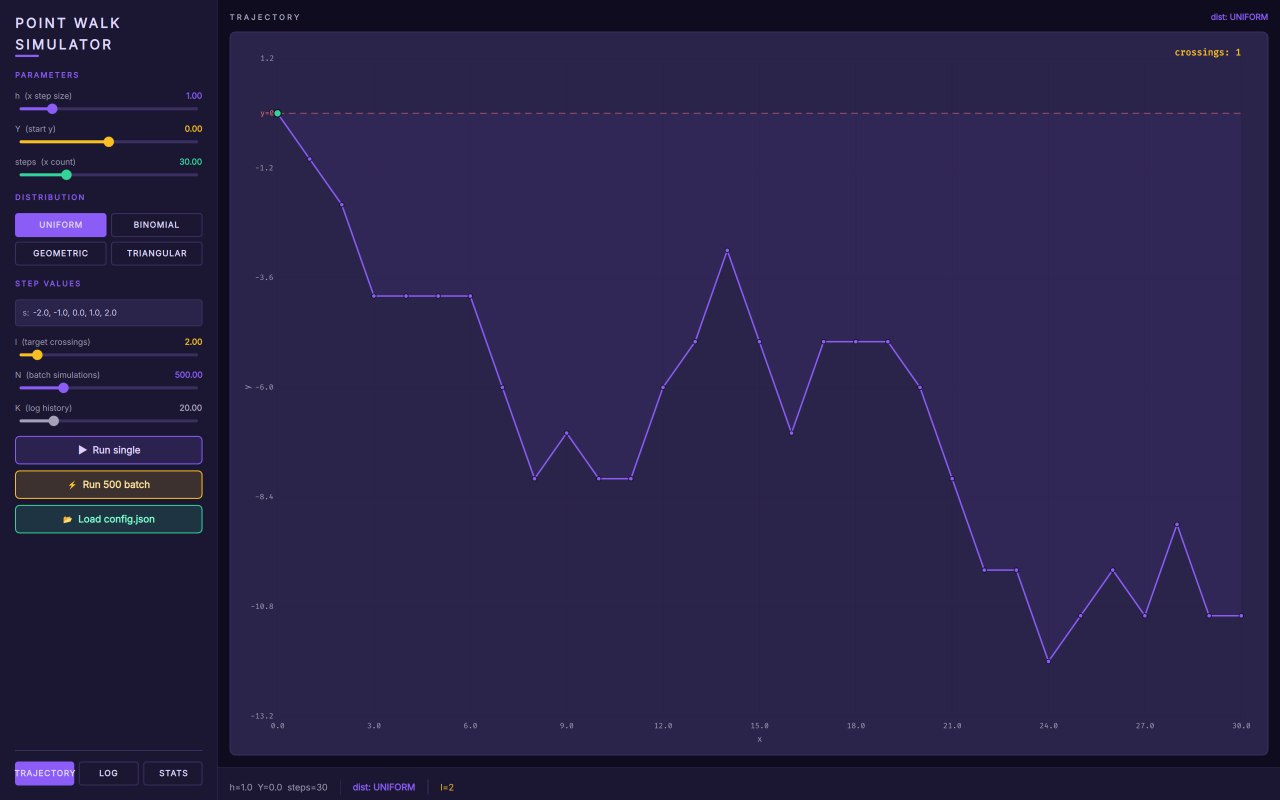
\includegraphics[width=0.8\textwidth]{assets/task04_gui.png}
\caption{Интерфейс приложения: панель управления и график траектории}
\end{figure}

\clearpage
\subsection{Задача 5. Кластеры и \(k\)-паттерны}
\label{sec:org62c3f2a}

Дана серия из \(M\) кластеров, каждый содержит \(n\) ячеек. В каждую ячейку помещается символ из алфавита \(A\) мощности \(r\). Лексема длины \(k\) называется \(k\)-паттерном. Два соседних кластера соединяемы по заданному \(k\)-паттерну, если конкатенация некоторого суффикса левого кластера с некоторым префиксом правого кластера в точности даёт этот паттерн.
\subsubsection{Модель и критерий соединяемости}
\label{sec:orgd9cc949}

Кластеры \(C_i\) и \(C_{i+1}\) соединяемы по паттерну \(P\) длины \(k\), если существуют натуральные \(a\) и \(b\) такие, что:

$$a + b = k, \quad 1 \le a \le n-1, \quad 1 \le b \le n-1$$
$$\operatorname{suffix}_a(C_i) \oplus \operatorname{prefix}_b(C_{i+1}) = P$$

Здесь \(\oplus\) --- оператор конкатенации строк.
\subsubsection{Алгоритм проверки соединяемости}
\label{sec:orga2dd359}

\begin{listing}[htbp]
\caption{Метод проверки соединяемости двух соседних кластеров}
\begin{minted}[]{cpp}
bool ClusterSimulator::are_connected(
    const std::string& left,
    const std::string& right) const {
    for (int a = 1; a < m_cells_per_cluster
              && a < m_pattern_length; ++a) {
        int b = m_pattern_length - a;
        if (b < 1 || b >= m_cells_per_cluster) continue;

        std::string suffix = left.substr(
            m_cells_per_cluster - a, a);
        std::string prefix = right.substr(0, b);

        if (suffix + prefix == m_pattern) return true;
    }
    return false;
}
\end{minted}
\end{listing}
\subsubsection{Генерация кластеров}
\label{sec:org8611ead}

Кластеры генерируются побуквенно методом обратного преобразования, согласно заданному распределению вероятностей на алфавите.

\begin{listing}[htbp]
\caption{Генерация одного кластера}
\begin{minted}[]{cpp}
std::string ClusterSimulator::generate_cluster() {
    std::string cluster;
    for (int i = 0; i < m_cells_per_cluster; ++i) {
        double r = m_distribution(m_generator);
        for (size_t j = 0; j < m_cumulative.size(); ++j) {
            if (r < m_cumulative[j]) {
                cluster += m_symbols[j];
                break;
            }
        }
    }
    return cluster;
}
\end{minted}
\end{listing}
\subsubsection{Результаты моделирования}
\label{sec:orge21bf09}

Эксперименты проведены при \(M = 10\), \(n = 5\), \(k = 3\), \(A = \{0, 1\}\), \(C = 10^6\).

В первом эксперименте с равномерным распределением (\(P(0)=P(1)=0.5\)) и паттерном \(101\) распределение числа соединяемых пар \(D\) близко к симметричному с максимумом в точке \(D = 3\): \(P(D=3) \approx 0.275\), на краях \(P(D=0) \approx 0.039\) и \(P(D=7) \approx 0.001\) (\(P(D=8) \approx 0.000\)). Вероятность одновременной соединяемости всех девяти пар составляет \(P_{\text{all}} \approx 0.039\).

При смещённом распределении (\(P(1) = 0.7\), паттерн \(101\)) соединяемость резко возрастает: \(P_{\text{all}} \approx 0.182\), максимум смещается в область больших \(D\) (\(P(D=6) \approx 0.290\)), а вероятность малых \(D\) становится пренебрежимо малой (\(P(D=0) \approx 0.001\)).

Паттерн \(111\) при равномерном распределении практически не даёт соединяемых пар: \(P_{\text{all}} \approx 0.000\), а с вероятностью \(P(D \le 2) \approx 0.990\) соединяемыми оказываются не более двух пар из рядом стоящих кластеров; значения \(D \ge 4\) практически не наблюдаются.

При равномерном распределении и паттерне \(101\) распределение \(D\) близко к симметричному с максимумом в \(D = 3\). При смещённом распределении (\(P(1) = 0.7\)) вероятность всех соединяемых пар резко возрастает. Паттерн \(111\) при равномерном распределении практически не даёт соединяемых пар.

\clearpage
\subsection{Задача 6. Ступенчатая фигура}
\label{sec:orgaa98f19}

Дан отрезок \([0; M]\), \(M > 0\), разбитый на отрезки длины \(h\). На каждом подотрезке определена случайная величина \(\xi\), принимающая значения из множества \(\{0, \tau, 2\tau, \ldots, n\tau\}\).
\subsubsection{Математическая модель}
\label{sec:org53b62ef}

$$f(x) = \xi_i, \quad x \in (x_{i-1}, x_i], \quad i = 1, \ldots, N$$

Ступенчатая фигура называется \textbf{строго возрастающей лестницей}, если \(\xi_1 < \xi_2 < \cdots < \xi_N\).

\begin{listing}[htbp]
\caption{Генерация одного значения \(\xi_i\)}
\begin{minted}[]{cpp}
double StaircaseSimulation::sample_one() {
    int n = m_cfg.n_values;
    double tau = m_cfg.tau;

    switch (m_cfg.dist) {
    case Distribution::Uniform: {
        std::uniform_int_distribution<int> d(0, n);
        return d(m_rng) * tau;
    }
    case Distribution::Binomial: {
        std::binomial_distribution<int>
            d(m_cfg.binom_trials, m_cfg.binom_p);
        int k = d(m_rng);
        return (k % (n + 1)) * tau;
    }
    case Distribution::FiniteGeometric: {
        std::vector<double> weights(n + 1);
        double sum = 0.0;
        for (int i = 0; i <= n; i++) {
            weights[i] = std::pow(1.0 - m_cfg.geom_p, i)
                        * m_cfg.geom_p;
            sum += weights[i];
        }
        for (auto& w : weights) w /= sum;
        std::discrete_distribution<int>
            d(weights.begin(), weights.end());
        return d(m_rng) * tau;
    }
    case Distribution::DiscreteTriangular: {
        double a = m_cfg.tri_a, peak = m_cfg.tri_b, c = m_cfg.tri_c;
        if (a >= c) {
            std::uniform_int_distribution<int> d(0, n);
            return d(m_rng) * tau;
        }
        peak = std::max(a, std::min(peak, c));
        std::uniform_real_distribution<double> u01(0.0, 1.0);
        double u = u01(m_rng);
        double Fc = (peak - a) / (c - a);
        double sample;
        if (u < Fc)
            sample = a + std::sqrt(u * (c - a) * (peak - a));
        else
            sample = c - std::sqrt((1.0 - u) * (c - a) * (c - peak));
        int best = static_cast<int>(
            std::round((sample - a) / (c - a) * n));
        best = std::max(0, std::min(best, n));
        return best * tau;
    }
    }
    return 0.0;
}
\end{minted}
\end{listing}
\subsubsection{Графический интерфейс}
\label{sec:orgcece3aa}

Приложение построено на Qt6 Quick. Боковая панель содержит настройки параметров и область статистики. Сгенерированные ступенчатые фигуры отображаются на сетке по 6 штук на страницу с пагинацией.

\begin{figure}[H]
\centering
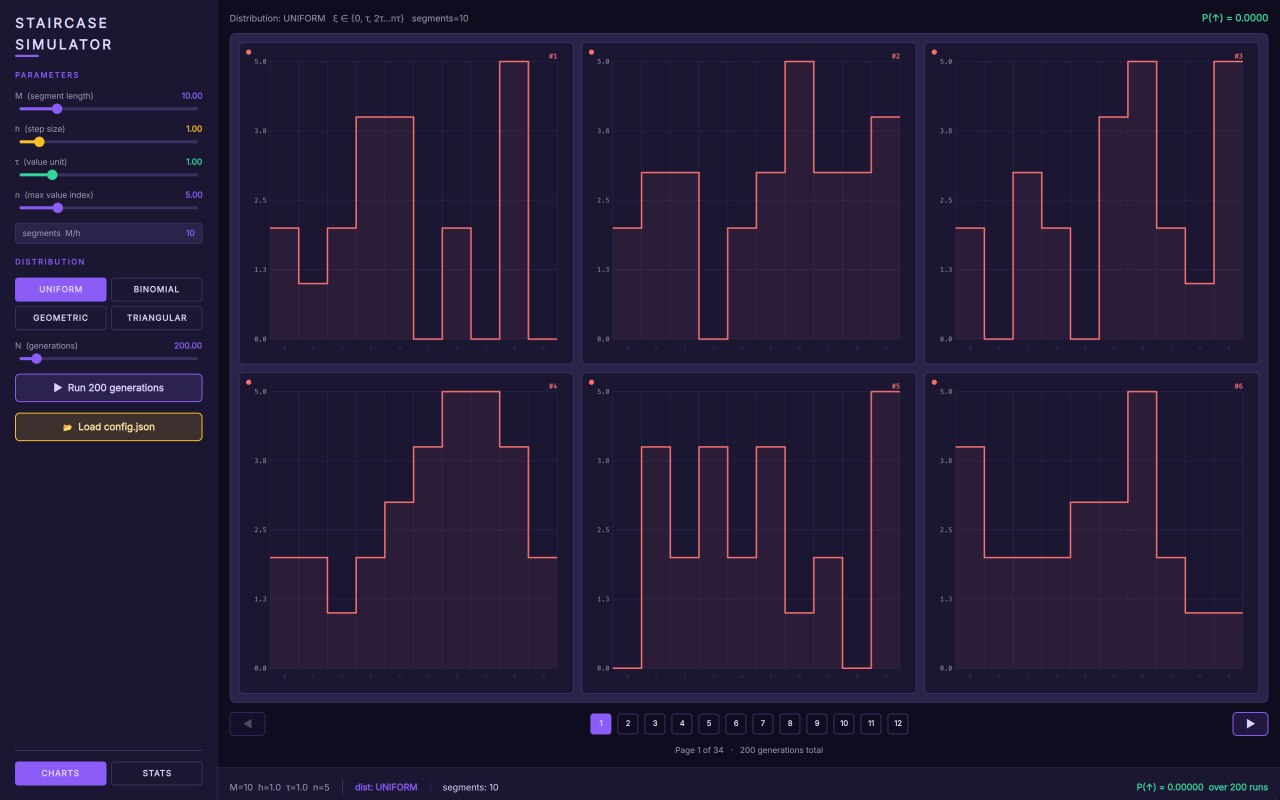
\includegraphics[width=0.8\textwidth]{assets/task06_gui.png}
\caption{Интерфейс приложения: панель управления, статистика и сетка фигур}
\end{figure}

\clearpage
\subsection{Задача 7. Комплексная плоскость и случайные блуждания с фиксированным шагом}
\label{sec:org72730e8}

Рассматривается случайное блуждание на комплексной плоскости с фиксированной длиной шага. Направление каждого шага выбирается из конечного набора равноотстоящих углов.
\subsubsection{Математическая модель}
\label{sec:orge175fc5}

$$\begin{cases} x_k = x_{k-1} + \rho \cos\!\big(\frac{2\pi}{n}\xi_k\big) \\[4pt] y_k = y_{k-1} + \rho \sin\!\big(\frac{2\pi}{n}\xi_k\big) \end{cases} \qquad (x_0, y_0) = (0, 0)$$

Поддерживаются четыре закона распределения индекса \(\xi_k\): равномерное, биномиальное, усечённое геометрическое и дискретное треугольное.

Блуждание считается вернувшимся в начало координат, если \(\|z_k\| = \sqrt{x_k^2 + y_k^2} < \varepsilon\).
\subsubsection{Ядро симуляции}
\label{sec:org58a3f11}

\begin{listing}[htbp]
\caption{Метод симуляции одного блуждания}
\begin{minted}[]{cpp}
WalkResult ComplexWalkSimulation::run_single() {
    WalkResult r;
    r.path.push_back({0.0, 0.0});
    for (int step = 1; step <= m_cfg.K; step++) {
        int xi = sample_xi();
        double dx = m_cfg.rho
            * std::cos(2.0 * M_PI / m_cfg.n * xi);
        double dy = m_cfg.rho
            * std::sin(2.0 * M_PI / m_cfg.n * xi);
        Point2D pt{r.path.back().x + dx,
                   r.path.back().y + dy};
        r.path.push_back(pt);
        if (std::hypot(pt.x, pt.y) < m_cfg.epsilon) {
            r.returned = true;
            r.return_step = step;
            return r;
        }
    }
    r.returned = false;
    r.return_step = -1;
    return r;
}
\end{minted}
\end{listing}

\begin{listing}[htbp]
\caption{Генерация индекса направления для треугольного распределения}
\begin{minted}[]{cpp}
int ComplexWalkSimulation::sample_xi_triangular() {
    double u = std::uniform_real_distribution<double>(
        0.0, 1.0)(m_rng);
    double fc = (m_cfg.tri_c - m_cfg.tri_a);
    double fb = (m_cfg.tri_b - m_cfg.tri_a) / fc;
    double s;
    if (u <= fb) {
        s = m_cfg.tri_a
          + std::sqrt(u * fc * (m_cfg.tri_b - m_cfg.tri_a));
    } else {
        s = m_cfg.tri_c
          - std::sqrt((1.0 - u) * fc
                      * (m_cfg.tri_c - m_cfg.tri_b));
    }
    int idx = static_cast<int>(
        s / fc * (m_cfg.n - 1) + 0.5);
    return std::clamp(idx, 0, m_cfg.n - 1);
}
\end{minted}
\end{listing}
\subsubsection{Графический интерфейс}
\label{sec:orgd4a2ecc}

Приложение построено на Qt6 Quick. Левая панель содержит органы управления параметрами; правая область отображает траекторию или статистику. Визуализация на комплексной плоскости с координатной сеткой и маркерами начала/конца. Траектории, вернувшиеся в начало, выделяются зелёным цветом.

\begin{figure}[H]
\centering
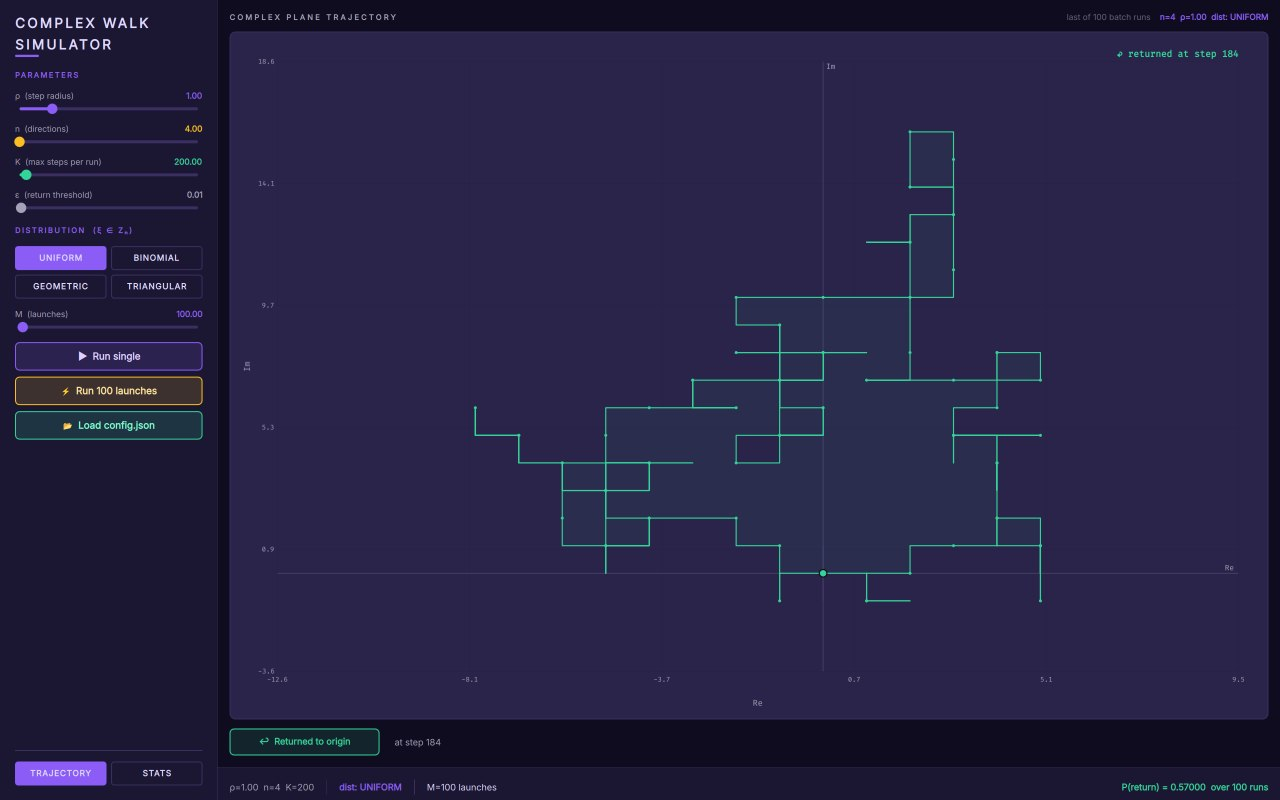
\includegraphics[width=0.8\textwidth]{assets/task07_gui.png}
\caption{Интерфейс приложения: панель управления и траектория на комплексной плоскости}
\end{figure}

\clearpage
\subsection{Задача 8. Моделирование взрыва бочки с бензином}
\label{sec:orged1e82e}

Рассматривается вероятностная модель разрушения бочки с бензином при многократном обстреле. Каждый выстрел независимо поражает цель с заданной вероятностью. Бочка взрывается при двух и более попаданиях; при одном попадании взрыв происходит с дополнительной условной вероятностью.
\subsubsection{Математическая модель}
\label{sec:orgaa5fbb5}

Производится \(n\) независимых выстрелов по бочке. Число попаданий \(X\) имеет биномиальное распределение:

$$P(X = k) = \binom{n}{k} p^k (1-p)^{n-k}$$

Бочка взрывается при \(X \ge 2\) (гарантированный взрыв) и при \(X = 1\) с вероятностью \(p_1\).
\subsubsection{Программная реализация}
\label{sec:orge2c9e51}

Задача реализована в виде консольного приложения, использующего шаблонный класс \texttt{TaskRunner}.

\begin{listing}[htbp]
\caption{Полная программа моделирования взрыва бочки}
\begin{minted}[]{cpp}
static void print_usage(const char* prog) {
    std::println("Usage:");
    std::println("  {} <p> <p1> <n> <simulations>", prog);
}

int main(int argc, char** argv) {
    if (argc != 5) { print_usage(argv[0]); return 1; }

    double p  = std::strtod(argv[1], nullptr);
    double p1 = std::strtod(argv[2], nullptr);
    int    n  = std::strtol(argv[3], nullptr, 10);
    size_t sim = static_cast<size_t>(
        std::strtoull(argv[4], nullptr, 10));

    auto experiment = [p, p1, n](auto& rng) {
        std::bernoulli_distribution hit(p);

        int hits = 0;
        for (int i = 0; i < n; i++) {
            if (hit(rng)) ++hits;
        }

        if (hits == 0) return false;
        if (hits >= 2) return true;

        return std::bernoulli_distribution(p1)(rng);
    };

    TaskRunner runner;
    auto results = runner.run(experiment, sim);

    auto counts = tally(results);
    std::print("P(barrel explodes) = {:.6f}\n",
               static_cast<double>(counts[true]) / sim);
    std::print("P(barrel survives) = {:.6f}\n",
               static_cast<double>(counts[false]) / sim);
    return 0;
}
\end{minted}
\end{listing}

\begin{figure}[H]
\centering
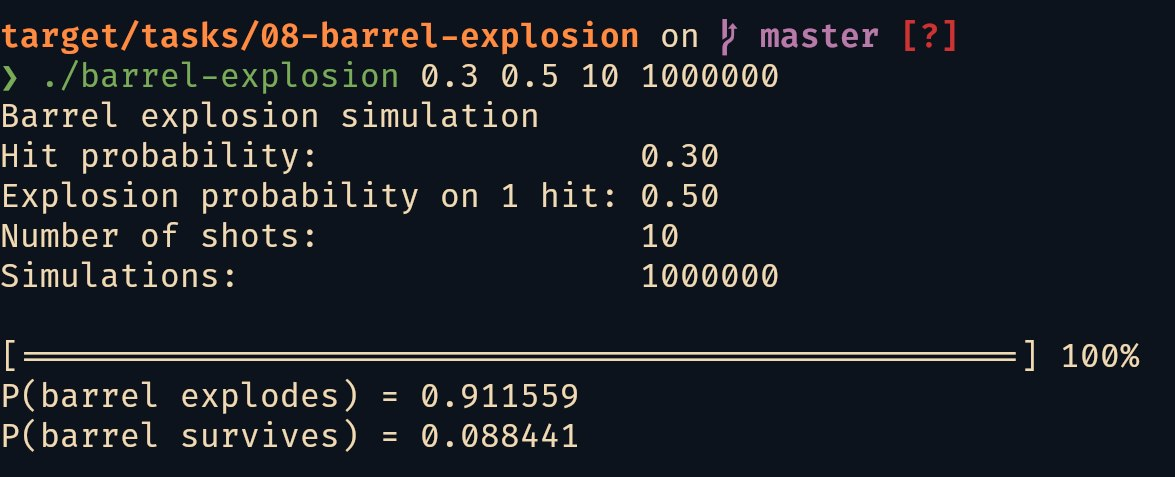
\includegraphics[width=0.9\textwidth]{assets/task08.png}
\caption{Результат моделирования взрыва бочки для \(p = 0{,}3\), \(p_1 = 0{,}5\), \(n = 10\)}
\end{figure}

\clearpage
\subsection{Задача 9. Криптоанализ: совершенная секретность и теорема Шеннона}
\label{sec:orgd7746ac}

Рассматривается задача криптоанализа --- оценка совершенной секретности шифров на малом пространстве сообщений и ключей.
\subsubsection{Математическая модель}
\label{sec:orgf596be6}

Задано конечное пространство сообщений \(T = \{m_1, \ldots, m_{|T|}\}\) с априорным распределением \(P(M = m)\) и пространство ключей \(K = \{k_1, \ldots, k_{|K|}\}\) с распределением \(P(Key = k)\). Шифрование выполняется детерминированной функцией \(c = E_k(m)\).

Рассматриваются два алгоритма шифрования:

$$c_i = (m_i + k^{(i \bmod |k|)}) \bmod 26 \quad \text{(Виженер)}$$

$$c_i = (m_i \oplus k^{(i \bmod |k|)}) \bmod 26 \quad \text{(Вернам)}$$

где \(k^{(t)}\) --- \$t\$-й символ ключа \(k \in K\), а \(|k|\) --- длина ключа.

\textbf{Шенноновская совершенная секретность.} Шифр обладает совершенной секретностью, если для всех \(m \in T\), \(c \in C\):

$$P(M = m | C = c) = P(M = m)$$
\subsubsection{Программная реализация}
\label{sec:org84028c4}

Анализ выполняется полным перебором всех пар «сообщение---ключ».

\begin{listing}[htbp]
\caption{Функция анализа}
\begin{minted}[]{cpp}
void analyze(
    const std::vector<std::string>& msgs,
    const std::vector<double>& msg_probs,
    const std::vector<std::string>& keys,
    const std::vector<double>& key_probs,
    const std::string& target_cipher,
    const std::string& target_msg,
    bool use_vigenere)
{
    auto encrypt = [&](const std::string& m, const std::string& k) {
        return use_vigenere
                   ? vigenere_encrypt(m, k)
                   : vernam_encrypt(m, k);
    };

    std::map<std::string, double> p_cipher;
    std::map<std::string, std::map<std::string, double>>
        p_cipher_given_msg;

    for (size_t j = 0; j < msgs.size(); ++j)
        for (size_t s = 0; s < keys.size(); ++s) {
            std::string c = encrypt(msgs[j], keys[s]);
            p_cipher[c] += msg_probs[j] * key_probs[s];
            p_cipher_given_msg[msgs[j]][c] += key_probs[s];
        }

    double pm = 0.0;
    for (size_t j = 0; j < msgs.size(); ++j)
        if (msgs[j] == target_msg) {
            pm = msg_probs[j];
            break;
        }

    double pc = p_cipher.count(target_cipher) > 0
                    ? p_cipher.at(target_cipher)
                    : 0.0;
    double pcm =
        (p_cipher_given_msg.count(target_msg) > 0 &&
         p_cipher_given_msg.at(target_msg)
             .count(target_cipher) > 0)
            ? p_cipher_given_msg.at(target_msg)
                  .at(target_cipher)
            : 0.0;
    double pmc = (pc > 0.0) ? (pcm * pm / pc) : 0.0;

    std::println("  P(Cipher='{}')             = {:.4f}",
                 target_cipher, pc);
    std::println("  P(Cipher='{}'|M='{}') = {:.4f}",
                 target_cipher, target_msg, pcm);
    std::println("  P(M='{}'|Cipher='{}') = {:.4f}",
                 target_msg, target_cipher, pmc);
    std::println("  Perfect secrecy?           = {}",
                 std::abs(pmc - pm) < 1e-9 ? "YES" : "NO");
}
\end{minted}
\end{listing}

\begin{listing}[htbp]
\caption{Функции шифрования Виженера и Вернама}
\begin{minted}[]{cpp}
std::string vigenere_encrypt(
    const std::string& msg, const std::string& key)
{
    std::string out(msg.size(), 'a');
    for (size_t i = 0; i < msg.size(); i++)
        out[i] = 'a' + (msg[i] - 'a'
                 + key[i % key.size()] - 'a') % 26;
    return out;
}

std::string vernam_encrypt(
    const std::string& msg, const std::string& key)
{
    std::string out(msg.size(), 'a');
    for (size_t i = 0; i < msg.size(); i++)
        out[i] = 'a' + ((msg[i] - 'a')
                 ^ (key[i % key.size()] - 'a')) % 26;
    return out;
}
\end{minted}
\end{listing}

Программа тестирует четыре сценария: шифр Виженера и шифр Вернама с равномерным и неравномерным распределением ключей. Шифр Вернама с равномерным распределением ключей удовлетворяет условию совершенной секретности; шифр Виженера --- нет.

\begin{figure}[H]
\centering
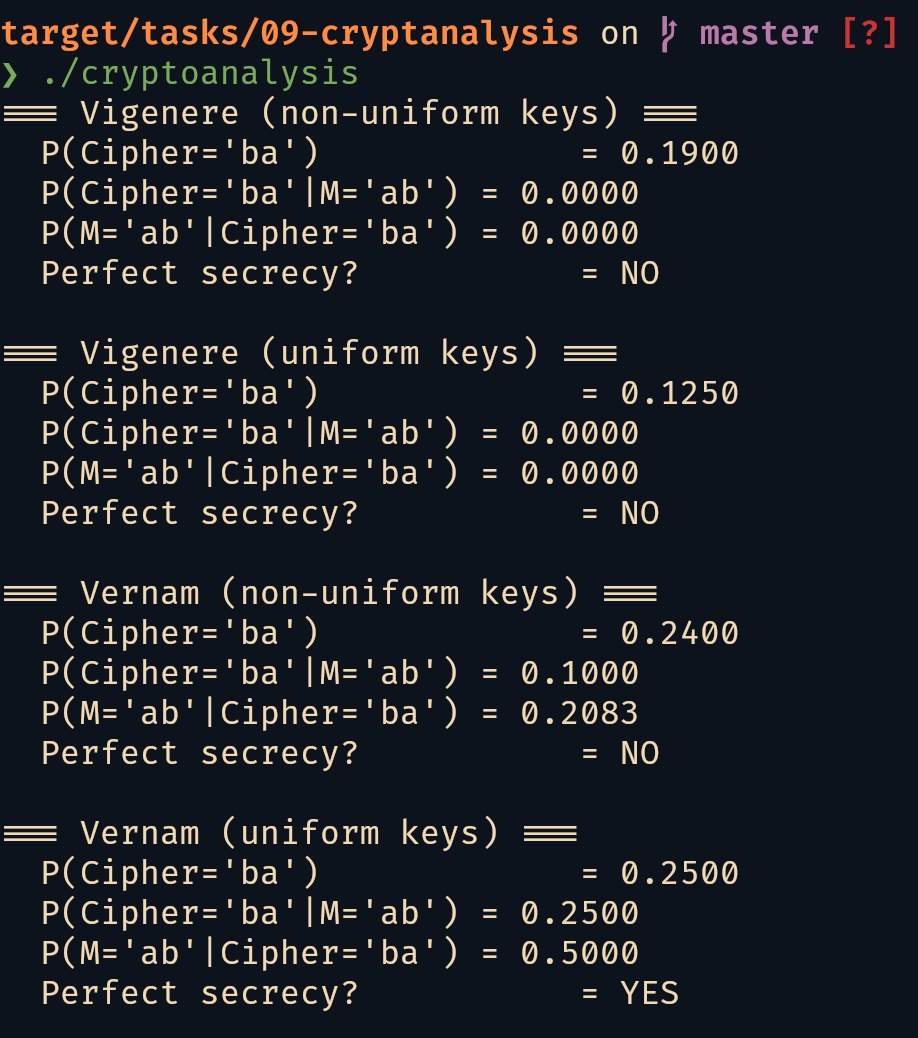
\includegraphics[width=0.9\textwidth]{assets/task09.png}
\caption{Результат криптоанализа: вывод программы для всех четырёх сценариев}
\end{figure}

\clearpage
\subsection{Задача 10. Подбрасывание монеты из кошелька: байесовская вероятностная модель}
\label{sec:org29191c4}

Рассматривается байесовская задача: в кошельке находится \(n\) монет, ровно \(k\) из которых --- двуглавые (обе стороны — «орёл»). Наугад выбирается одна монета и подбрасывается 4 раза. Требуется оценить условную вероятность того, что четвёртый бросок выпадет «орлом» при условии, что первые три броска также дали «орла».
\subsubsection{Математическая модель}
\label{sec:org0569392}

Пусть \(D\) --- событие «выбрана двуглавая монета», \(F\) --- событие «выбрана честная монета». Априорные вероятности:

$$P(D) = \frac{k}{n}, \qquad P(F) = \frac{n - k}{n}$$

$$P(\text{4-й орёл} \mid \text{первые 3 орла}) = \frac{P(4H)}{P(3H)} = \frac{15k + n}{2(7k + n)}$$

Частные случаи: \(k = 0\) --- \(P = 1/2\); \(k = n\) --- \(P = 1\); \(n = 10, k = 3\) --- \(P = 55/62 \approx 0{,}8871\).
\subsubsection{Программная реализация}
\label{sec:org36ac410}

\begin{listing}[htbp]
\caption{Полная программа оценки условной вероятности}
\begin{minted}[]{cpp}
int main(int argc, char** argv) {
    if (argc != 4) {
        std::println("Usage: {} <n> <k> <experiments>", argv[0]);
        return 1;
    }

    int n = std::stoi(argv[1]);
    int k = std::stoi(argv[2]);
    size_t sim = std::stoull(argv[3]);

    auto experiment = [n, k](auto& rng)
        -> std::pair<bool, bool>
    {
        std::uniform_int_distribution<int> coin_dist(0, n - 1);
        std::bernoulli_distribution fair(0.5);

        int coin = coin_dist(rng);
        bool double_headed = (coin < k);

        bool t1 = double_headed ? true : fair(rng);
        bool t2 = double_headed ? true : fair(rng);
        bool t3 = double_headed ? true : fair(rng);
        bool t4 = double_headed ? true : fair(rng);

        bool first_three = t1 && t2 && t3;
        return {first_three, first_three && t4};
    };

    TaskRunner runner;
    auto results = runner.run(experiment, sim);

    size_t three_heads = 0, four_heads = 0;
    for (auto [cond, full] : results) {
        if (cond)  three_heads++;
        if (full)  four_heads++;
    }

    std::print("P(4th heads | first 3 heads) = {:.6f}\n",
               1.0 * four_heads / three_heads);
    return 0;
}
\end{minted}
\end{listing}

\begin{figure}[H]
\centering
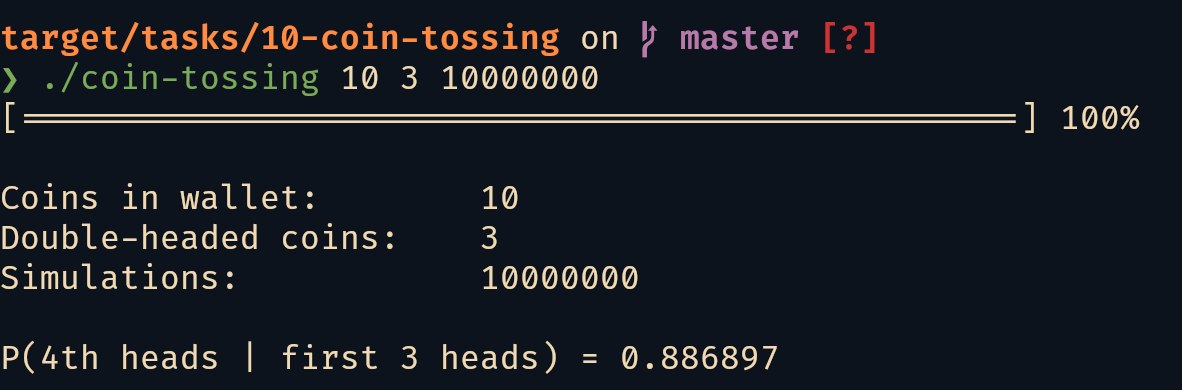
\includegraphics[width=0.9\textwidth]{assets/task10.png}
\caption{Результат моделирования для \(n = 10\), \(k = 3\), \(10^7\) испытаний}
\end{figure}

\clearpage
\subsection{Задача 11. Дискретная случайная величина и её числовые характеристики}
\label{sec:orgbee1801}

Разработана библиотека для работы с произвольными дискретными случайными величинами. Программа вычисляет числовые характеристики и визуализирует их.
\subsubsection{Математическая модель}
\label{sec:orgf95a881}

Дискретная случайная величина \(X\) задаётся множеством пар «значение---вероятность»: \(\{(x_1, p_1), (x_2, p_2), \ldots, (x_n, p_n)\}\).

При задании случайной величины обязано выполняться условие нормировки --- сумма всех вероятностей должна равняться единице:

$$\sum_{i=1}^{n} p_i = 1, \quad p_i > 0, \quad x_i \neq x_j \ \ (i \neq j)$$

$$\mu = \mathbb{E}[X] = \sum_{i=1}^{n} x_i \cdot p_i$$

$$\sigma^2 = \mathbb{D}[X] = \sum_{i=1}^{n} (x_i - \mu)^2 \cdot p_i$$

$$\gamma_1 = \frac{\mathbb{E}[(X - \mu)^3]}{\sigma^3} = \frac{\sum_{i=1}^{n} (x_i - \mu)^3 \cdot p_i}{\sigma^3}$$

$$\gamma_2 = \frac{\mathbb{E}[(X - \mu)^4]}{\sigma^4} - 3 = \frac{\sum_{i=1}^{n} (x_i - \mu)^4 \cdot p_i}{\sigma^4} - 3$$

Для независимых дискретных случайных величин \(X\) и \(Y\) определены сумма (свёртка) и произведение:

$$P(X + Y = z) = \sum_{x_i + y_j = z} p_i \cdot q_j$$

$$P(X \cdot Y = z) = \sum_{x_i \cdot y_j = z} p_i \cdot q_j$$

\clearpage
\subsubsection{Программная реализация}
\label{sec:orgddc4ff5}

\begin{listing}[htbp]
\caption{Интерфейс класса DiscreteRandomVariable}
\begin{minted}[]{cpp}
class DiscreteRandomVariable {
public:
    DiscreteRandomVariable(
        std::vector<std::pair<double, double>> data);

    std::vector<std::pair<double, double>> pmf() const;
    std::vector<std::pair<double, double>> cdf() const;

    double expectation() const;
    double variance() const;
    double skewness() const;
    double kurtosis() const;

    DiscreteRandomVariable operator+(
        const DiscreteRandomVariable& other) const;
    DiscreteRandomVariable operator*(
        const DiscreteRandomVariable& other) const;
    DiscreteRandomVariable operator*(double scalar) const;

    void normalize();
    void save_to_file(const std::string& path) const;
    static DiscreteRandomVariable load_from_file(
        const std::string& path);

private:
    std::map<double, double> m_data;
    void validate() const;
};
\end{minted}
\end{listing}

Приложение построено на GLFW + ImGui + ImPlot и визуализирует три графика: столбчатую диаграмму PMF, ступенчатую CDF и полигон распределения.

\begin{figure}[H]
\centering
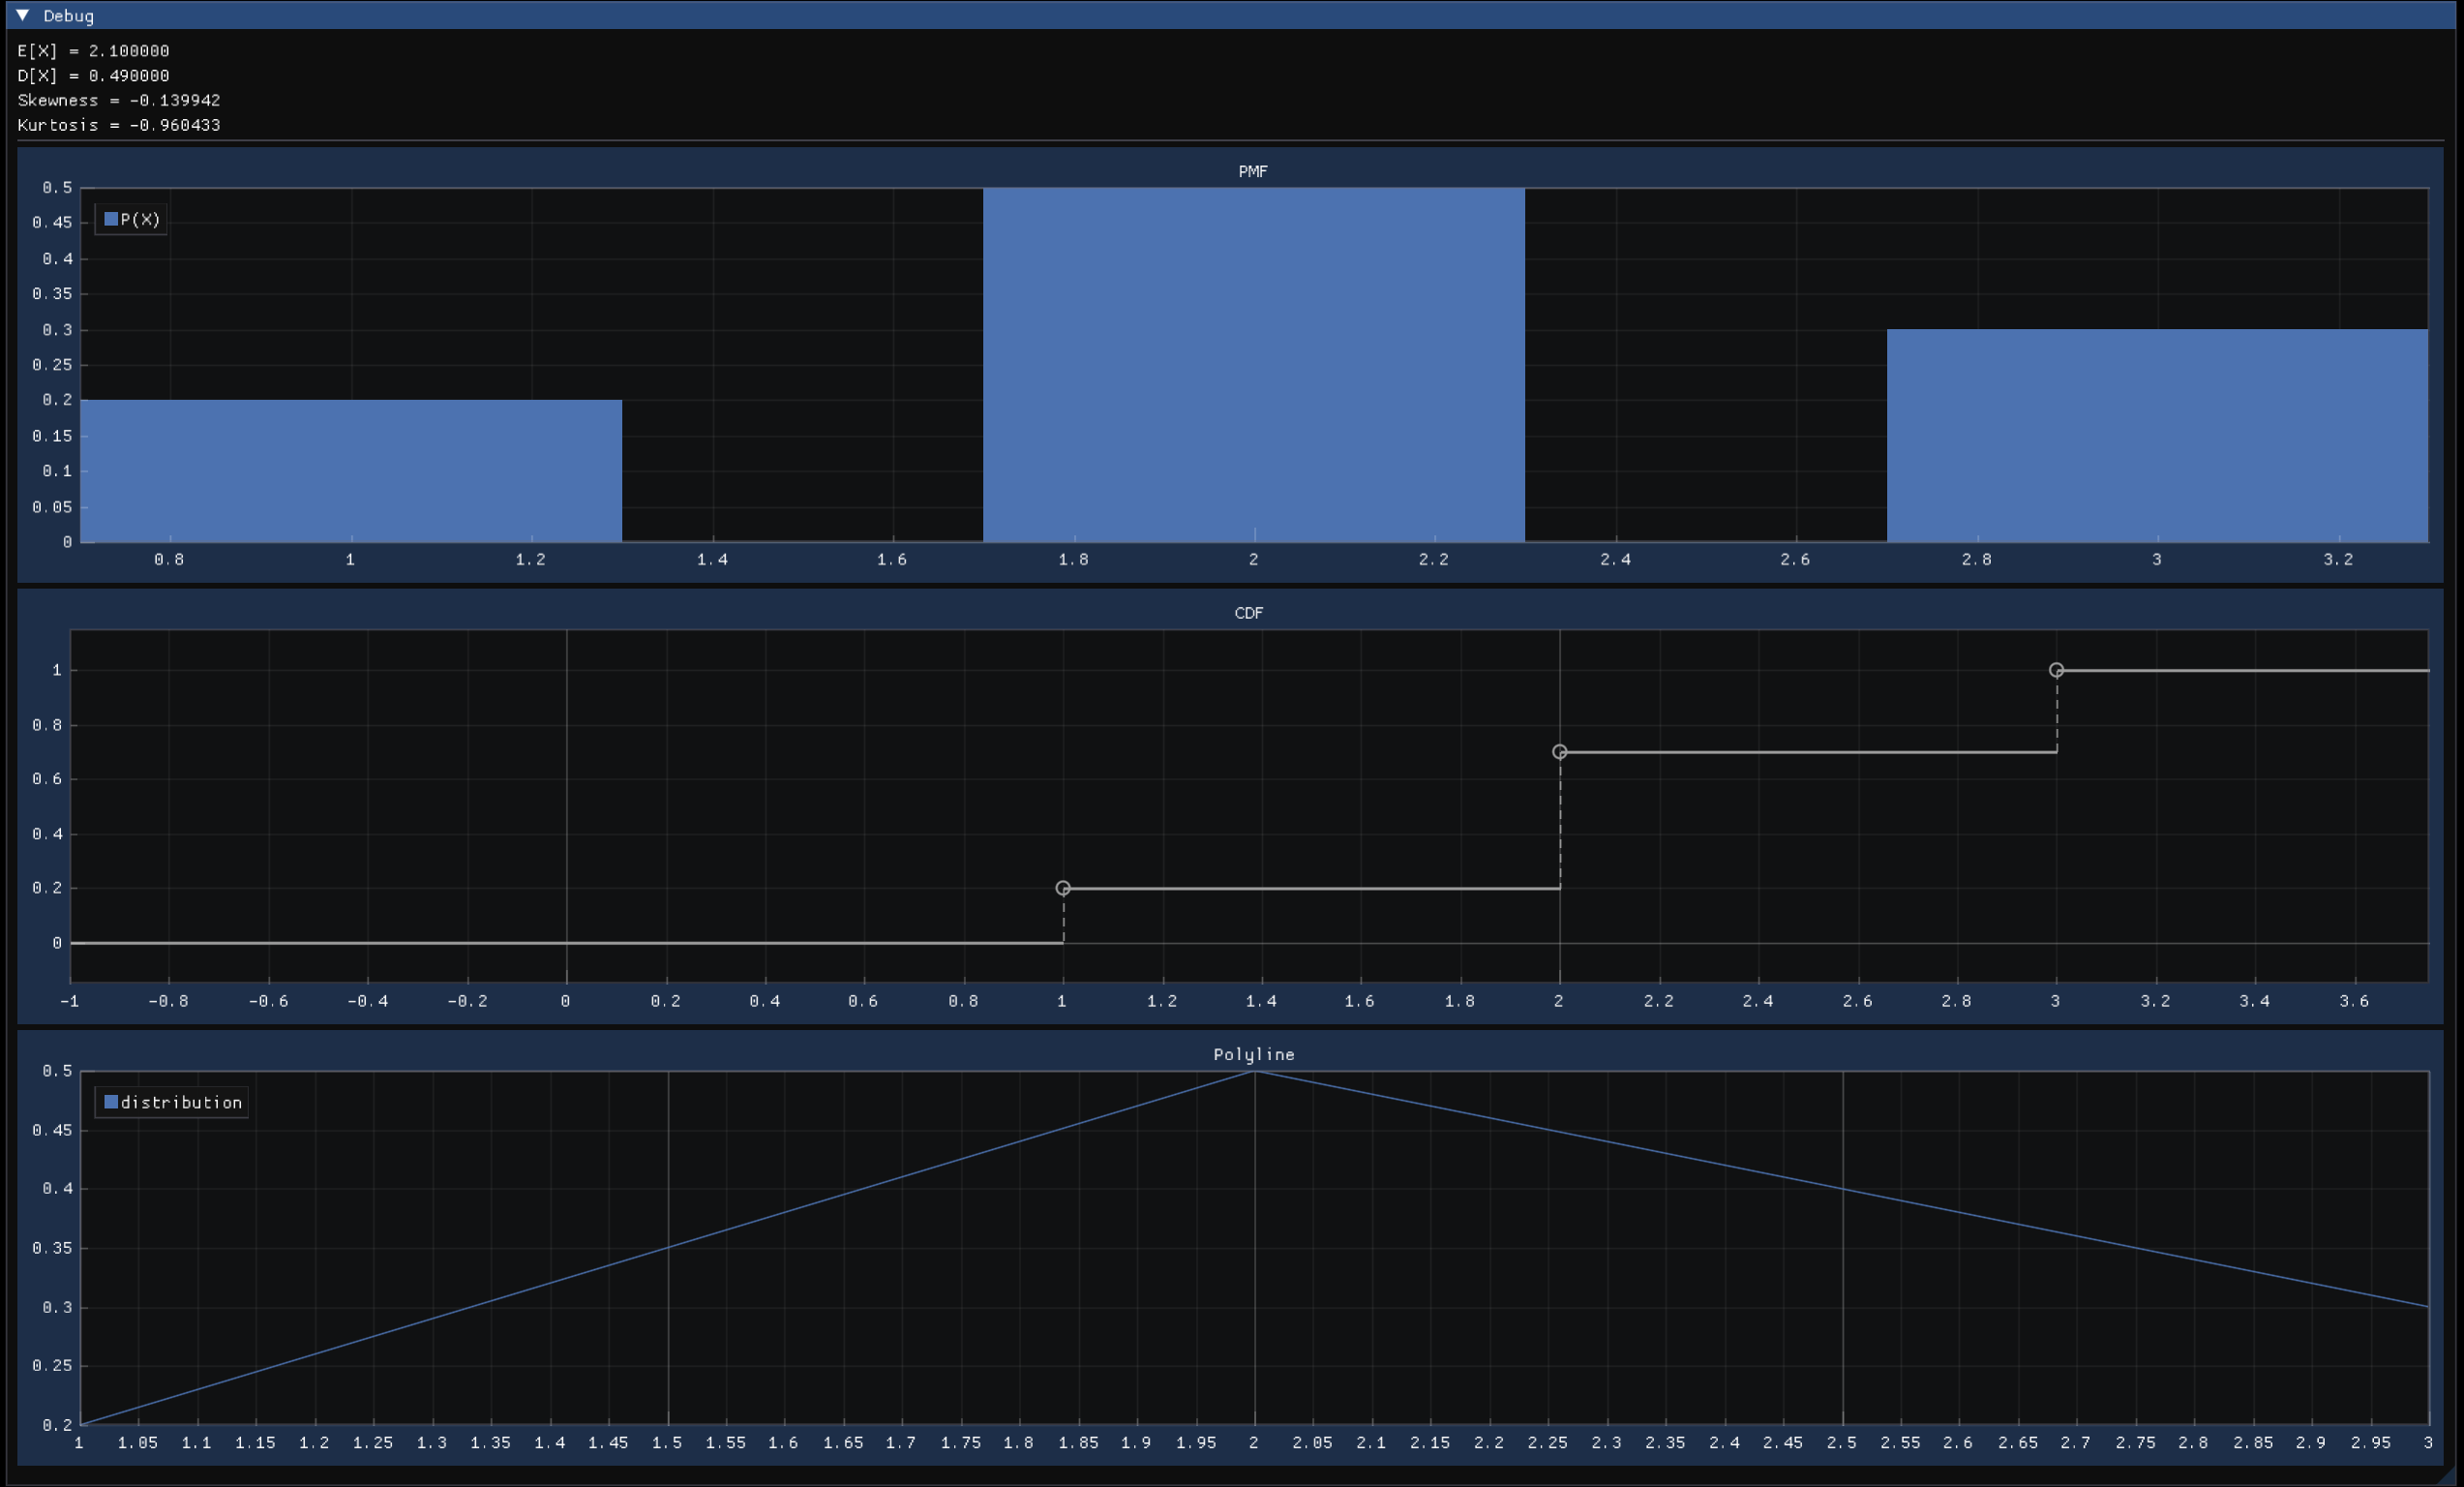
\includegraphics[width=0.9\textwidth]{assets/task11.png}
\caption{Визуализация дискретной случайной величины: PMF, CDF и полигон распределения}
\end{figure}

\clearpage
\subsection{Задача 12. Моделирование Бюффона}
\label{sec:org7a015de}

Реализована классическая задача Бюффона о бросании иглы на плоскость с параллельными линиями. Методом Монте-Карло оценивается вероятность пересечения иглой линии.
\subsubsection{Ядро симуляции}
\label{sec:org8a822e5}

\begin{listing}[htbp]
\caption{Класс NeedleSimulation}
\begin{minted}[]{cpp}
struct NeedleResult {
    double x;
    double phi;
    bool crosses;
};

class NeedleSimulation {
public:
    NeedleSimulation(double d, double L);
    NeedleResult run_single();
    std::vector<NeedleResult> run_batch(int n);
private:
    double m_d, m_L;
    std::mt19937 m_rng;
    std::uniform_real_distribution<double> m_dist_x;
    std::uniform_real_distribution<double> m_dist_phi;
};
\end{minted}
\end{listing}

\begin{listing}[htbp]
\caption{Бросок одной иглы}
\begin{minted}[]{cpp}
NeedleResult NeedleSimulation::run_single() {
    double x   = m_dist_x(m_rng);
    double phi = m_dist_phi(m_rng);
    bool crosses = x <= (m_L / 2.0) * std::sin(phi);
    return {x, phi, crosses};
}
\end{minted}
\end{listing}
\subsubsection{Графический интерфейс}
\label{sec:org2049b63}

Приложение построено на Qt6 Quick и предоставляет два режима работы.

\textbf{Пакетный режим.} Пользователь задаёт число бросаний \(N\) (100---100~000) и запускает симуляцию.

\textbf{Визуальный режим.} Каждая игла отображается на холсте: пересекающие линии иглы окрашиваются красным, не пересекающие --- фиолетовым.

\begin{figure}[H]
\centering
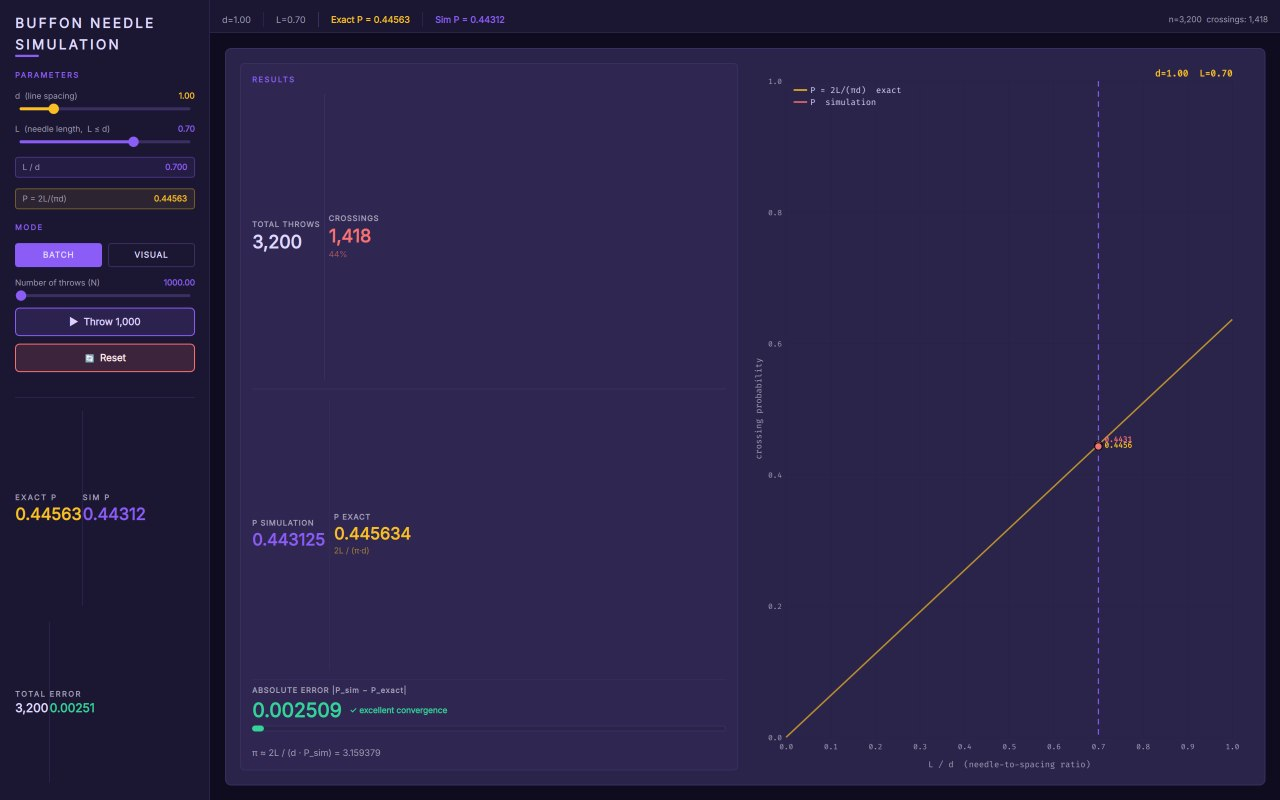
\includegraphics[width=0.8\textwidth]{assets/task12_gui.png}
\caption{Интерфейс приложения в пакетном режиме}
\end{figure}

\begin{figure}[H]
\centering
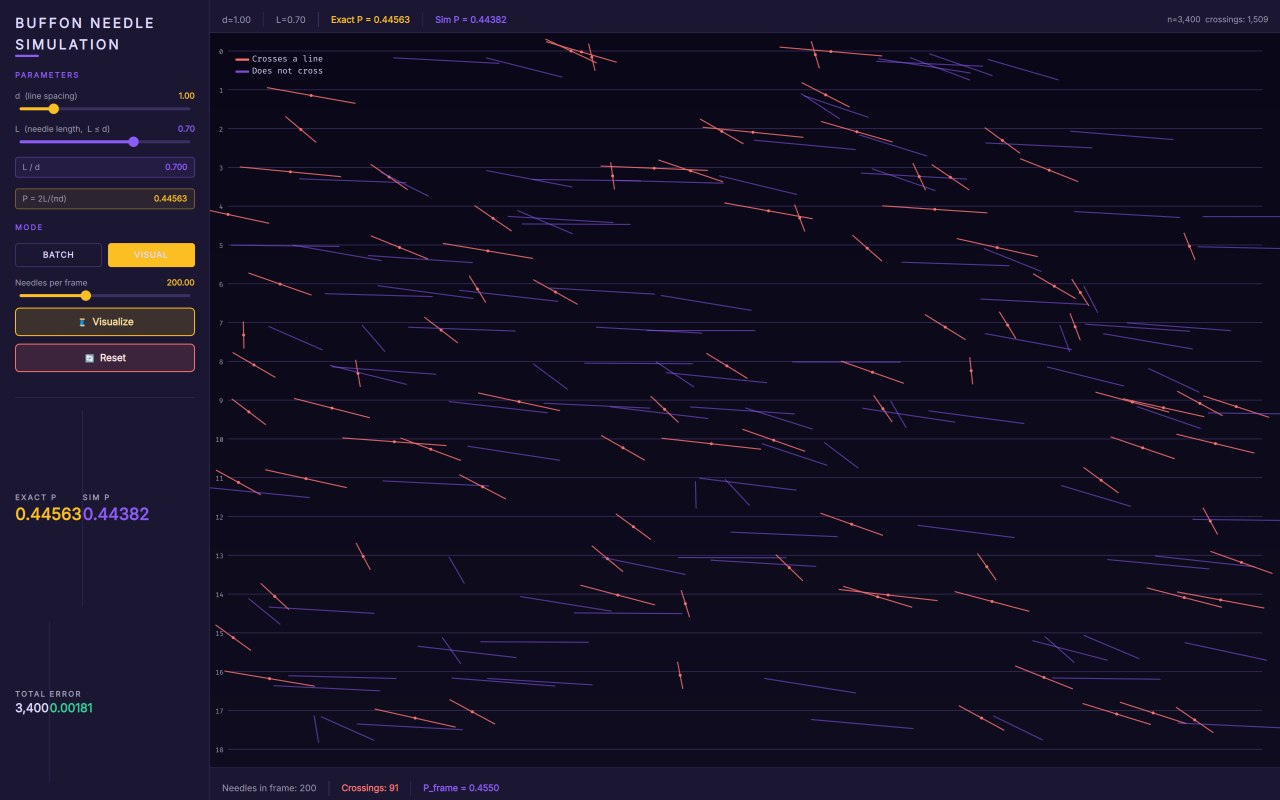
\includegraphics[width=0.8\textwidth]{assets/task12_visual.png}
\caption{Визуальный режим: пересекающие (красные) и не пересекающие (фиолетовые) иглы}
\end{figure}

\clearpage
\subsection{Задача 13. Статистический анализ случайных графов}
\label{sec:org2e963e9}

Разработана программа для генерации случайных взвешенных графов и вычисления набора графовых характеристик методом Монте-Карло. На основе JSON-конфигурации программа порождает \(N\) графов, вычисляет для каждого набор метрик и агрегирует результаты. Симуляция параллелизуется по аппаратным потокам.
\subsubsection{Математическая модель}
\label{sec:org6825b27}

Генерируется неориентированный взвешенный граф \(G = (V, E)\) с \(|V| = n\) вершинами, где \(n \in \mathbb{N}\) --- параметр конфигурации. Множество возможных рёбер образуют все неупорядоченные пары вершин \((i, j)\), \(i < j\); всего таких пар \(C_n^2 = n(n-1)/2\). Для каждой пары независимо разыгрываются наличие ребра и его вес.

Сначала определяется, существует ли ребро: из равномерного распределения извлекается \(u \sim U(0, 1)\), и ребро объявляется присутствующим, если \(u < d\); в противном случае \(w_{ij} = 0\) и ребра нет. Существующему ребру присваивается целый вес, равномерно распределённый на множестве \(\{1, 2, \ldots, L\}\) (по условию задачи \(L = 10\), хотя конфигурация допускает и другие значения). Итоговая схема генерации:

$$w_{ij} = \begin{cases} U\{1, 2, \ldots, L\}, & U(0,1) < d, \\ 0, & \text{иначе}, \end{cases} \qquad P(e_{ij} \neq 0) = d$$

Параметр \(d\) называется плотностью графа и представляет собой вероятность наличия отдельного ребра. Число рёбер \(m\) имеет биномиальное распределение \(m \sim \mathrm{Bin}(C_n^2, d)\) с математическим ожиданием \(\mathbb{E}[m] = d \cdot n(n-1)/2\), поэтому фактическая плотность конкретного графа \(m/C_n^2\) флуктуирует вокруг \(d\). При \(d = 1\) граф является полным, при \(d = 0\) --- пустым. Вес ребра не влияет на его наличие и разыгрывается независимо.

Для каждого сгенерированного графа вычисляются следующие характеристики:

\begin{center}
\begin{tabular}{lll}
Метрика & Алгоритм & Сложность\\
\hline
Вес минимального остовного дерева & Прима & \(O(n^2)\)\\
Длина макс. цикла по рёбрам & DFS & \(O(n!)\)\\
Число рёбер макс. цикла по весам & DFS & \(O(n!)\)\\
Изолированные вершины & Перебор & \(O(n^2)\)\\
Остовные деревья & Алгоритм Барейсса & \(O(n^3)\)\\
Компоненты связности & BFS & \(O(n^2)\)\\
Кликовые компоненты & BFS + проверка & \(O(n^2+m)\)\\
\end{tabular}
\end{center}
\subsubsection{Алгоритмы вычисления метрик}
\label{sec:orgd92e254}

\textbf{Сумма весов рёбер минимального остовного дерева.} Остовное дерево связного графа --- это подграф без циклов, содержащий все его вершины; вес остовного дерева равен сумме весов входящих в него рёбер. Минимальное остовное дерево строится жадным алгоритмом Прима: множество уже включённых вершин последовательно дополняется вершиной, соединённой с деревом ребром минимального веса:

$$A = \text{MST}(G) = \sum_{v \in V} \min_{u \in S,\, (u,v) \in E} w(u, v),$$

где \(S\) --- множество вершин, уже включённых в MST. Алгоритм поддерживает массив \texttt{key[v]} --- минимальный вес ребра, соединяющего \(v\) с текущим деревом, --- и массив \texttt{in\_mst[v]} --- флаг включения вершины. На каждом шаге выбирается непомеченная вершина с минимальным ключом, её ключ добавляется к общему весу, после чего ключи всех её соседей обновляются. Если граф несвязен, минимальный ключ на очередном шаге равен \texttt{kInf}, и цикл прерывается. Благодаря матричному представлению графа сложность составляет \(O(n^2)\).

\begin{listing}[htbp]
\caption{Алгоритм Прима для вычисления веса MST}
\begin{minted}[]{cpp}
i32 mst_weight(const Graph& g) {
  i32 n = g.n;
  if (n <= 1) return 0;

  constexpr i32 kInf = std::numeric_limits<i32>::max();
  i32 key[n];
  bool in_mst[n];
  for (i32 i = 0; i < n; i++) {
    key[i] = kInf;
    in_mst[i] = false;
  }
  key[0] = 0;

  i32 total = 0;
  for (i32 iter = 0; iter < n; iter++) {
    i32 u = -1;
    for (i32 v = 0; v < n; v++)
      if (!in_mst[v] && (u == -1 || key[v] < key[u]))
        u = v;

    if (key[u] == kInf) break;
    in_mst[u] = true;
    total += key[u];

    for (i32 v = 0; v < n; v++) {
      if (!in_mst[v] && edge_exists(g, u, v)) {
        i32 w = static_cast<i32>(edge_weight(g, u, v));
        if (w < key[v]) key[v] = w;
      }
    }
  }
  return total;
}
\end{minted}
\end{listing}

Граф хранится в виде сжатой верхне-треугольной матрицы смежности: элементы \(w_{ij}\) для всех пар \(0 \le i < j < n\) упакованы в \texttt{std::span<u8>}, доступ к ребру выполняется по индексу за \(O(1)\). Нулевой вес означает отсутствие ребра.

\textbf{Поиск максимального цикла.} Длина цикла это --- число его рёбер, вес \(W(C) = \sum_{(i,j) \in C} w_{ij}\) --- сумма весов ребер цикла. Задача о самом длинном простом цикле является NP-complete, поэтому решается программно полным перебором. Из всех найденных циклов удерживаются длина самого большого по числу рёбер цикла и число рёбер самого большого по сумме весов цикла. Число простых путей в худшем случае растёт как \(O(n!)\), поэтому метод применим только при небольших \(n\).

\begin{listing}[htbp]
\caption{Поиск максимального цикла}
\begin{minted}[]{cpp}
struct CycleDfs {
  const Graph& g;
  bool* visited;
  i32 path_len;
  i32 best_edges;
  i32 best_weight_edges;
  i32 best_weight;
};

static void dfs(CycleDfs& s, i32 v, i32 start, i32 depth,
                i32 weight_so_far) {
  s.visited[v] = true;
  s.path_len++;

  for (i32 u = 0; u < s.g.n; u++) {
    if (u == v || !edge_exists(s.g, v, u)) continue;
    i32 w = static_cast<i32>(edge_weight(s.g, v, u));

    if (u == start && depth >= 2) {
      i32 cycle_edges = s.path_len;
      i32 cycle_weight = weight_so_far + w;
      if (cycle_edges > s.best_edges)
        s.best_edges = cycle_edges;
      if (cycle_weight > s.best_weight) {
        s.best_weight = cycle_weight;
        s.best_weight_edges = cycle_edges;
      }
      continue;
    }

    if (!s.visited[u])
      dfs(s, u, start, depth + 1, weight_so_far + w);
  }

  s.path_len--;
  s.visited[v] = false;
}

CycleStats find_cycle_stats(const Graph& g) {
  i32 n = g.n;
  bool visited[n];

  CycleDfs s{.g = g, .visited = visited, .path_len = 0,
             .best_edges = 0, .best_weight_edges = 0,
             .best_weight = 0};

  for (i32 start = 0; start < n; start++) {
    for (i32 i = 0; i < n; i++) visited[i] = false;
    s.path_len = 0;
    dfs(s, start, start, 0, 0);
  }

  return CycleStats{.longest_by_edges = s.best_edges,
                    .edge_count_of_heaviest = s.best_weight_edges};
}
\end{minted}
\end{listing}

\textbf{Количество остовных деревьев.} Число \(F = \tau(G)\) вычисляется по матричной теореме Кирхгофа: оно равно определителю редуцированной матрицы Лапласа \(L'\) размера \((n-1) \times (n-1)\), получаемой из матрицы Кирхгофа удалением последней строки и столбца:

$$L'_{ij} = \begin{cases} \deg(i), & i = j, \\ -1, & (i,j) \in E, \\ 0, & \text{иначе} \end{cases}$$

Определитель находится алгоритмом Барейсса:

$$a_{i,j}^{(k+1)} = \frac{a_{i,j}^{(k)} \cdot a_{k,k}^{(k)} - a_{i,k}^{(k)} \cdot a_{k,j}^{(k)}}{a_{k-1,k-1}^{(k-1)}}$$

Если в ходе исключения на главной диагонали встретился ноль, граф несвязен и \(\tau(G) = 0\). Сложность \(O(n^3)\).

\begin{listing}[htbp]
\caption{Подсчёт остовных деревьев методом Барейсса}
\begin{minted}[]{cpp}
i64 count_spanning_trees(const Graph& g) {
  i32 n = g.n;
  if (n <= 1) return 1;

  i32 m = n - 1;
  std::vector<std::vector<i64>> a(m, std::vector<i64>(m, 0));

  for (i32 i = 0; i < m; i++) {
    i64 degree = 0;
    for (i32 k = 0; k < n; k++)
      if (k != i && edge_exists(g, i, k))
        degree++;

    a[i][i] = degree;

    for (i32 j = 0; j < m; j++) {
      if (i == j) continue;
      a[i][j] = edge_exists(g, i, j) ? -1 : 0;
    }
  }

  i64 prev = 1;
  for (i32 k = 0; k < m; k++) {
    if (a[k][k] == 0) return 0;
    for (i32 i = k + 1; i < m; i++)
      for (i32 j = k + 1; j < m; j++)
        a[i][j] = (a[i][j] * a[k][k] -
                   a[i][k] * a[k][j]) / prev;
    prev = a[k][k];
  }
  return a[m - 1][m - 1];
}
\end{minted}
\end{listing}

\textbf{Компоненты связности, изолированные вершины и полные подграфы.} Компоненты связности находятся поиском в ширину. Каждая вершина обрабатывается один раз, сложность \(O(n^2)\).

\textbf{Вершина называется изолированной}, если её степень равна нулю; число таких вершин подсчитывается перебором строк матрицы смежности за \(O(n^2)\).

\textbf{Количество компонент связности, являющихся полными подграфами исходного графа.} компонента является полным подграфом, если любая пара её вершин соединена ребром. Для каждой найденной компоненты перебираются все пары её вершин; если хотя бы одна пара не соединена, компонента полным подграфом не является. Суммарная сложность проверки --- \(O(n^2 + m)\), где \(m\) --- число рёбер графа.
\subsubsection{Программная реализация}
\label{sec:org684fa2f}

Приложение принимает JSON-конфигурацию и имя выходного файла. В выходной JSON для каждой выбранной метрики записываются выборочное среднее \texttt{mean} и дисперсия \texttt{variance}. Количество испытаний определяется уровнем точности: \texttt{low} (1000), \texttt{medium} (10,000), \texttt{high} (100,000), \texttt{extreme} (1,000,000).

\begin{listing}[htbp]
\caption{Пример конфигурационного файла}
\begin{minted}[]{json}
{
  "n": 10,
  "edge_length": 10,
  "graph_density": 0.99,
  "seed": 14527346871,
  "precision": "extreme",
  "metrics": {
    "mst_weight": true,
    "longest_cycle_edges": true,
    "heaviest_cycle_edges": true,
    "isolated_vertices": true,
    "spanning_trees": true,
    "connected_components": true,
    "clique_components": true
  }
}
\end{minted}
\end{listing}

Испытания распределяются между аппаратными потоками: диапазон испытаний делится на непересекающиеся чанки, каждый поток обрабатывает свой чанк с собственным генератором \texttt{mt19937} и локальными аккумуляторами, что исключает корреляцию последовательностей и синхронизацию при записи результатов. По завершении данных в чанке локальные накопленные суммы сливаются в глобальные под мьютексом. Память для очередного графа выделяется в аренном аллокаторе потока и освобождается сразу после обработки испытания.

\begin{figure}[H]
\centering
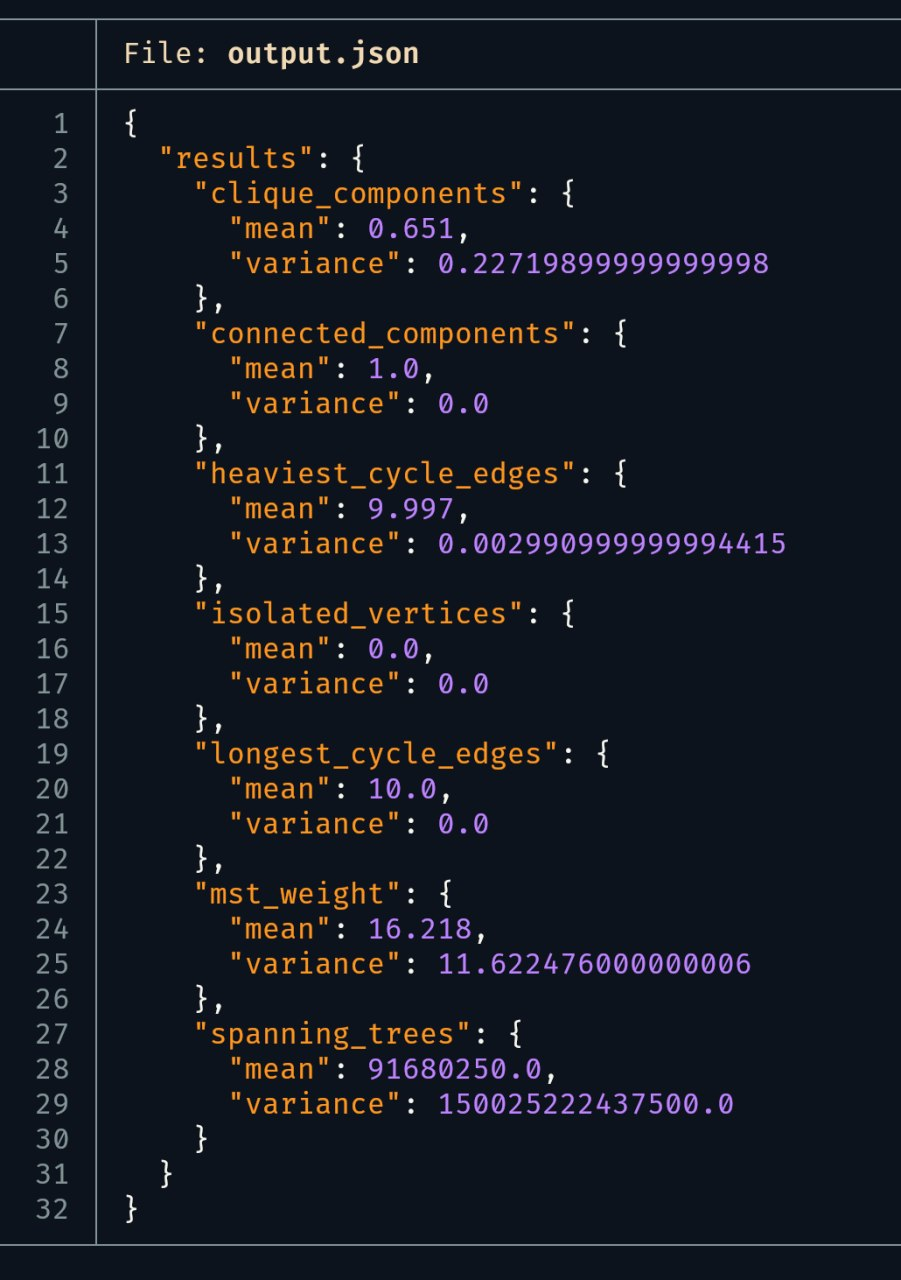
\includegraphics[width=0.9\textwidth]{assets/task13.png}
\caption{Результат статистического анализа случайного графа}
\end{figure}

\clearpage
\section{Вывод}
\label{sec:org20ff547}

В ходе курсовой работы была выполнена программная реализация задач вероятностного моделирования. Разработано 13 приложений на языке \texttt{C++23}, охватывающих широкий спектр вероятностных моделей.

Для каждого задания были разработаны математические модели, реализованы алгоритмы численного моделирования методом Монте-Карло и проведены вычислительные эксперименты. Полученные эмпирические результаты сопоставлены с аналитическими формулами, что подтвердило корректность реализаций.

Программная архитектура включает использование различных графических фреймворков и подходов к организации вычислений. Результаты работы демонстрируют эффективность вероятностных методов для решения задач вероятностного моделирования.

\clearpage
\section{Список использованных источников}
\label{sec:orgef87fd7}

\begin{enumerate}
\item Гмурман В.Е. Теория вероятностей и математическая статистика. --- Москва : Юрайт, 2023. --- 480 с.
\item Костиков Ю.А., Романенков А.М. Практикум по теории вероятности: случайное событие : методическое пособие для студентов. --- Москва : ВИНИТИ, 2010. --- 40 с.
\item Qt 6 Documentation [Электронный ресурс]. --- Режим доступа: \url{https://doc.qt.io/qt-6/} (дата обращения: 24.04.2026).
\item Cornut O. Dear ImGui: Bloat-free Graphical User Interface for C++ [Электронный ресурс]. --- Режим доступа: \url{https://github.com/ocornut/imgui} (дата обращения: 24.04.2026).
\item Lohmann N. JSON for Modern C++ (nlohmann/json) [Электронный ресурс]. --- Режим доступа: \url{https://github.com/nlohmann/json} (дата обращения: 24.04.2026).
\item CMake Documentation [Электронный ресурс]. --- Режим доступа: \url{https://github.com/Kitware/CMake} (дата обращения: 24.04.2026).
\item GLFW --- An OpenGL library [Электронный ресурс]. --- Режим доступа: \url{https://github.com/glfw/glfw} (дата обращения: 24.04.2026).
\item Pezent E. ImPlot: Immediate Mode Plotting for Dear ImGui [Электронный ресурс]. --- Режим доступа: \url{https://github.com/epezent/implot} (дата обращения: 24.04.2026).
\end{enumerate}

\clearpage
\section{Приложение}
\label{sec:orgdc69374}

Исходный код всех разработанных приложений, а также исходные тексты настоящей пояснительной записки в \texttt{pdf}, \texttt{org} и \texttt{tex} форматах доступны в репозитории:

\url{https://github.com/rgu-labs/term4-kursach}
\end{document}
